%%%%%%%%%%%%%%%%%%%%%%%%%%%%%%%%%%%%%%%%%%%%%%%%%%%%%%%%%%%%%%%%%%%%%%%%%%%%%%%
%
% IIT Sample THESIS File,   Version 3, Updated by Babak Hamidian on 11/18/2003
%
%%%%%%%%%%%%%%%%%%%%%%%%%%%%%%%%%%%%%%%%%%%%%%%%%%%%%%%%%%%%%%%%%%%%%%%%%%%%%%%
% File: sample3.tex                                   %
% IIT Sample LaTeX File                               %
% by Ozlem Kalinli on 05/30/2003                      %
% Revised by Babak Hamidian on 11/18/2003             %
%%%%%%%%%%%%%%%%%%%%%%%%%%%%%%%%%%%%%%%%%%%%%%%%%%%%%%%
%                                                     %
% This is a sample thesis document created using      %
% iitthesis.cls style file. The PDF output is also    %
% available for your reference. In this file, it has  %
% been illustrated how to make table of contents,     %
% list of tables, list of figures, list of symbols,   %
% bibliography, equations, enumerations, etc.         %
% You can find detailed instructions                  %
% for using the style file in Help.doc,               %
% TableHelp.doc, FigureHelp.doc, and                  %
% Bibliography.doc files.                             %
%                                                     %
%%%%%%%%%%%%%%%%%%%%%%%%%%%%%%%%%%%%%%%%%%%%%%%%%%%%%%%
% Note: The texts that are used in this sample3.tex   %
% file are irrelevant. They are just used to show     %
% you the style created by iitthesis style file.      %
%%%%%%%%%%%%%%%%%%%%%%%%%%%%%%%%%%%%%%%%%%%%%%%%%%%%%%%

\documentclass{iitthesis}

\input .tex
% Document Options:
%
% Note if you want to save paper when printing drafts,
% replace the above line by
%
%   \documentclass[draft]{iitthesis}
%
% See Help file for more about options.

\usepackage[dvips]{graphicx}    % This package is used for Figures
\usepackage{rotating}           % This package is used for landscape mode.
\usepackage{epsfig}
\usepackage{mathrsfs}



%\usepackage{amssymb, amsmath, amsthm, color,enumerate}
\usepackage{multirow}
\usepackage{url}
%\usepackage{algorithm}
\usepackage{mcode}
\usepackage{amsfonts,amsmath,amssymb,amsthm,color,enumerate,mathtools,bbm,booktabs,array,tikz,pifont,comment,multirow,url,graphicx,float,verbatim,mathrsfs}





%\usepackage[dvips]{graphicx}    % This package is used for Figures
%\usepackage{rotating}           % This package is used for landscape mode.
%\usepackage{epsfig}
%\usepackage{subfigure}          % These two packages, epsfig and subfigure, are used for creating subplots.
%% Packages are explained in the Help document.
%\usepackage{mathrsfs}
%\usepackage{mathptmx}       % selects Times Roman as basic font
%\usepackage{helvet}         % selects Helvetica as sans-serif font
%\usepackage{courier}        
%\usepackage{mathtools}% selects Courier as typewriter font
%\usepackage{commath}
%\usepackage{makeidx}         % allows index generation
%\usepackage{graphicx}        % standard LaTeX graphics tool
%\usepackage{stackengine}                 % when including figure files
%\usepackage{multicol}        % used for the two-column index
%\usepackage{amsthm}
%\usepackage{amsmath}
%\usepackage{amsfonts}
%\usepackage{amssymb}
%\usepackage{color}     % Do not use: colors will appear in gray scale!
%\usepackage{url}
%\usepackage{verbatim}
%\usepackage{cite}
%\usepackage{chemarrow}
%\usepackage{listings}
% \usepackage{alltt}
% \usepackage{mcode}
% \usepackage{booktabs}
% \usepackage{array}
%\newcolumntype{L}{>{\centering\arraybackslash}m{3cm}}
%\usepackage[autolinebreaks]{mcode}
\input Ljiangdef.tex
%
%\newcommand{\bbz}{{\bf z}}
%\newcommand{\bbx}{{\bf x}}
%\newcommand{\bby}{{\bf y}}
%\newcommand{\bbX}{{\bf X}}
%\newcommand{\bbY}{{\bf Y}}
%\newcommand{\bbH}{{\bf H}}
%\newcommand{\bbB}{{\bf B}}
%\newcommand{\bbA}{{\bf A}}
%\newcommand{\bbalpha}{\boldsymbol\alpha}
%\newcommand{\bbbeta}{\boldsymbol\beta}
%\newcommand{\bbc}{{\bf c}}
%\newcommand{\bba}{{\bf a}}
%\newcommand{\bbb}{{\bf b}}
%\newcommand{\bbh}{{\bf h}}
%\newcommand{\bbn}{{\bf n}}
%\newcommand{\bbd}{{\bf d}}
%\newcommand{\vgamma}{\boldsymbol\gamma}
%\newcommand{\veczero}{\mathbf{0}}
%\newcommand{\EE}{\mathbb{E}}
%\newcommand{\NN}{\mathbb{N}}
%\newcommand{\DD}{\mathcal {D}}
%\newcommand{\RR}{\mathcal {R}}
%\newcommand{\PP}{\mathcal {P}}
%\newcommand{\HH}{\mathcal {H}}
%\newcommand{\FF}{\mathcal {F}}
%\newcommand{\XX}{\mathcal {X}}
%\newcommand{\QQ}{\mathbb {Q}}
%\newcommand{\FFF}{\mathbb {F}}
%\newcommand{\UU}{\mathbb{U}}
%\newcommand{\Order}{\mathcal O}
%\newcommand{\wup}{{\mathcal U}}
%\newcommand{\ccup}{{\mathcal C}}
%\newcommand{\reals}{\mathbb{R}}
%\def\abs#1{\ensuremath{\left \lvert #1 \right \rvert}}
%\newcommand{\ip}[3][{}]{\ensuremath{\left \langle #2, #3 \right \rangle_{#1}}}
%\newcommand{\ch}{\mathcal{H}}
%\newcommand{\fix}{\mathrm{fix}}
%\newcommand{\var}{\mathrm{var}}
%\newcommand{\spann}{\operatorname{span}}
%\newcommand{\eps}{\varepsilon}
%\newcommand{\bx}{{\mathbf x}}
%\newcommand{\by}{{\mathbf y}}
%\newcommand{\bz}{{\mathbf z}}
%\newcommand{\bc}{{\mathbf c}}
%\newcommand{\bv}{{\mathbf v}}
%\newcommand{\ba}{{\mathbf a}}
%\newcommand{\rad}{r^*}
%\newcommand{\XXX}{{\mathfrak X}}
%\newcommand{\rt}{k}
%\newcommand{\E}    {\operatorname{E}}
%\newcommand{\V}    {\operatorname{Var}}
%\newcommand{\err}  {\operatorname{error}}
%\newcommand{\cost} {\operatorname{cost}}
%\newcommand{\id}   {\operatorname{id}}
%\newcommand{\scp}[2]{\langle #1, #2 \rangle}
%
%\newcommand{\vx}{\boldsymbol{x}}
\DeclareMathOperator{\Yrand}{Yrand}
\newtheorem{theorem}{Theorem}[section]
\newtheorem{lemma}[theorem]{Lemma}
\newtheorem{proposition}[theorem]{Proposition}
\newtheorem{corollary}[theorem]{Corollary}
\newtheorem{algorithm}[theorem]{Algorithm}
%\newtheorem{defn}{Definition}[theorem]
\theoremstyle{definition}
\newtheorem{defn}[theorem]{Definition}
%\newcommand{\meanMCB}{\tt meanMCBer\_g}
%\newtheorem{corollary}{Corollary}[chapter]
%\newtheorem{definition}{Definition}[chapter]
%\newtheorem{remark}{Remark}[chapter]
%\newtheorem{proof}{Proof}[chapter]
%\renewcommand{\theenumi}{A\arabic{enumi}}
\begin{document}
% Define all the symbols used.

%%% Declarations for Title Page %%%
\title{Guaranteed Adaptive Monte Carlo Methods for Estimating Means of Random Variables}
\author{Lan Jiang}
\degree{Doctor of Philosophy} \dept{Applied Mathematics}
\date{May 2016}
%\copyrightnoticetrue      % crate copyright page or not
%\coadvisortrue           % add co-advisor. activate it by removing % symbol to add co-advisor
\maketitle                % create title and copyright pages


\prelimpages         % Settings of preliminary pages are done with \prelimpages command


%%%  Acknowledgement %%%
\begin{acknowledgement}     % acknowledgement environment, this is optional
\par  This dissertation could not have been written without Dr. Fred
J. Hickernell who not only served as my supervisor but also encouraged and challenged me throughout my academic program. He and the other faculty members, Dr. Greg Fasshauer, Dr. Lulu Kang and Dr. Hong Zhang guided me through the dissertation process, never accepting less than my best efforts. I appreciate the joint work with Dr. Art Owen and all the GAIL team members including Sou-Cheng Choi, Yuhan Ding, Yizhi Zhang, Llu{\'i}s Antoni Jim{\'e}nez Rugama and Xin Tong. I would also like to thank my husband Xuan Zhou for his support. I thank them all. 
\end{acknowledgement}


% Table of Contents
\tableofcontents
 \clearpage

% List of Tables
\listoftables

\clearpage

%List of Figures
\listoffigures

\clearpage



%%% Abstract %%%
\begin{abstract}% abstract environment, this is optional

${\mathbf x}$ Monte Carlo is a versatile computational method that may be used to approximate the means, $\mu$, of random variables, $Y$, whose distributions are not known explicitly. This thesis investigates how to reliably construct fixed width confidence intervals for $\mu$ with some prescribed absolute error tolerance $\varepsilon_a$, relative error tolerance $\varepsilon_r$ or some generalized error criterion. To facilitate this, it is assumed that the kurtosis, $\kappa$, of the random variable, $Y$, does not exceed a user specified bound $\kmax$. The key idea is to confidently estimate the variance of $Y$ by applying Cantelli's Inequality. A Berry-Esseen Inequality makes it possible to determine the sample size required to construct such a confidence interval. When relative error is involved, this requires an iterative process.  This idea for computing $\mu = \e(Y)$ can be used to develop a numerical integration by writing the integral as $\mu = \e (f(\vx)) = \int_{\reals^d}f(\vx)\rho(\vx)\dif\vx$, where $\vx$ is a $d$ dimensional random vector with probability density function $\rho$. A similar idea is used to develop an algorithm for computing $p = \e(Y)$ where $Y$ is a Bernoulli random variable. All of the algorithms have been implemented in the Guaranteed Automatic Integration Library (GAIL).

\end{abstract}
\textpages     % Settings of text-pages are done with \textpages command
% Chapters are created with \Chapter{title} command
\Chapter{INTRODUCTION}\label{introduction}

\Section{Monte Carlo simulation}

Monte Carlo is a widely used simulation method that can be applied to evaluate means of random variables, perform numerical integration, estimate default probabilities, understand and control complex stochastic systems, price financial derivatives and solve other real world problems.

 In the case of estimating the mean, $\mu$, of a random variable, $Y$, i.e.: $\mu = \e(Y)$, one generates $n$ independent and identically distributed (IID) $Y_i$ from the distribution of $Y$ and take the sample average, 
$$\mu \approx \hmu_n :=\frac1n\sum_{i=1}^nY_i.$$ The Strong Law of Large Numbers ensures that the sample mean converges to the true solution almost surely, i.e.: $\lim_{n \to \infty} \hmu_n =\mu \text{ a.s.}$ \cite[Theorem 20.1]{JP04}.







In this thesis, we investigate the ways to estimate the mean, $\mu$, of a random variable, $Y$, that satisfies the fixed width confidence interval condition with some prescribed absolute error tolerance $\varepsilon_a$,  
\begin{align}\label{absCI}
\Pr(\abs{\mu-\hmu_n} \leq \varepsilon_a) \geq 1-\alpha,
\end{align}
or relative error tolerance $\varepsilon_r$,
\begin{align}\label{relCI}
\Pr\left(\abs{\mu-\hmu_n}\leq \varepsilon_r\right) \geq 1-\alpha,
\end{align}
or some generalized error criterion, $\tol(\varepsilon_a,\varepsilon_r \abs{\mu})$, which is defined in Definition \ref{def:tolfun},
\begin{align}\label{hybridCI}
\Pr\left(\abs{\mu-\tmu_n}\leq \tol\left(\varepsilon_a, \varepsilon_r\abs{\mu}\right)\right) \geq 1-\alpha.
\end{align}
assuming a bounded kurtosis of the random variable $Y$,
\begin{equation} \label{def:boundedkurtosis}
\kappa = \frac{\e[(Y-\mu)^4]}{\sigma^4} \le \kappa_{\max}.
\end{equation}
where $\kmax$ is some bound defined in Definition \ref{def:kmax}. 

\Section{Background}

The Central Limit Theorem (CLT) provides a way to construct an approximate confidence interval for the $\mu$ in terms of the sample mean assuming a known variance $\var(Y)$. However, this is an asymptotic result, which is, the proposed procedure attains the desired coverage level in the limit as $\varepsilon\to 0$ but does not provide coverage guarantees for fixed $\varepsilon>0$.  We want such fixed $\varepsilon$ guarantees. The existing theory of fixed width confidence interval may make distributional assumptions that are too strong. 
Stein \cite{stein45} proposed a similar two stage procedure, however, his result requires normally distributed data and has no relative error criterion involved. In Monte Carlo applications one typically does not have much information about the underlying distribution. The form of the distribution for $Y$ is generally not known, $\var(Y)$ is generally not  known, and $Y$ is not necessarily bounded. We are aiming to derive fixed width confidence intervals that do not require such assumptions.  

The width of a confidence interval tends to become smaller as the number $n$ of sampled
function values increases. In special circumstances, we can choose $n$ to get a confidence interval of at most the desired length and at least the desired coverage level, $1-\alpha$. For instance, if the variance, $\sigma^2=\var(Y)$, is known then an approach based on Chebyshev's Inequality is available, though the actual coverage will usually be much higher than the nominal level, meaning that much narrower intervals would have sufficed. Known variance in addition to a Gaussian distribution for $Y$ supports a fixed width confidence interval construction that is not too conservative. The CLT provides a confidence interval that is asymptotically correct, but our aim is for something that is definitely correct for finite sample sizes. Finally, conservative fixed width confidence intervals for means can be constructed for bounded random variables, by appealing to exponential inequalities such as Hoeffding's or Chernoff's inequality.  Unfortunately, $Y$ is often unbounded, e.g., in the case where it represents the payoff of a call option.

If the relevant variance or bound is unknown, then approaches based on sequential statistics \cite{Siegmund85} may be available.  In sequential methods one keeps increasing $n$ until the interval is narrow enough. Sequential confidence intervals require us to take account of the stopping rule when computing the confidence level. Unfortunately, all existing sequential methods are lacking in some aspects. 

Serfling and Wackerly \cite{SerflingaWackerlyb76} consider sequential confidence intervals for the mean (alternatively for the median) in parametric distributions, symmetric about their center point. The symmetry condition is not suitable for general
purpose Monte Carlo applications.

Chow and Robbins\cite{ChowRobbins65} develop a sequential sampling fixed width confidence interval procedure for the mean, but its guarantees are only asymptotic (as $\varepsilon \to 0$). \cite{MukhDatta96} give a procedure similar to Chow and Robbins's, and it has similar drawbacks.

Bayesian methods can support a fixed width interval containing $\mu$ with $1-\alpha$ posterior probability, and
Bayesian methods famously do not require one to account for stopping rules. They do however require strong distributional assumptions.

\Section{Numerical integration}

An important special case of computing $\mu=\e(Y)$ is when $Y = f(\vX)$ for some function $f:\reals^d \to \reals$ and some random vector $\vX$ with probability density function $\rho: \reals^d \to [0,\infty)$. One may then interpret the mean of $Y$ as the multidimensional integral
\begin{align*}
I= \mu(f) = \e(\vY) = \int_{\reals^d}f(\vX)\rho(\vX)\dif \vX.
\end{align*}
%Note that given the problem of evaluating $I = \int_{\reals^d}g(\vx)\dif\vx$, one must choose a probability density function $\rho$ for which one can easily generate random vectors $\vx$, then set $f = g/\rho$. The quantities $\sigma^2$ and $\kappa$ defined above can be written in terms of weighted $\mathcal{L}_p$ norms of $f$:
%\begin{align*}
%\norm[4]{f}:=\left\{ \int_{\reals^d}\abs{f(\vx)}^p\rho(\vx)\dif\vx\right\}^{1/p}, \quad \sigma^2 = \norm[2]{f-\mu}^2,\quad \kappa = \frac{\norm[4]{f-\mu}^4}{\norm[2]{f-\mu}^4}.
%\end{align*}
%For a given $g$, the choice of $\rho$ is not unique, and making an optimal choice belongs to the realm of the importance sampling. The assumption of bounded kurtosis in \eqref{def:boundedkurtosis} required by Algorithm \ref{alg:meanMCabsg} corresponds to an assumption that integrand $f$ lies in the cone of functions \cite{CDHHZ13}
%\begin{align*}
%C_{\kmax} = \left\{ f \in \mathcal{L}_4: \norm[4]{f-\mu(f)} \leq \kmax^{1/4} \norm[4]{f-\mu(f)}\right\}.
%\end{align*}
%This is in contrast to a ball of functions, which wound be the case if one was satisfying a bounded variance condition.
%An important case pf computing $\mu = \e(Y)$ arises in the situation where $Y=f(\vX)$ for some function 
%Suppose we want to evaluate the multidimensional integral with integrand $f:\reals^d \to \reals$ with respect to some probability density function $\rho: \reals^d \to [0,\infty)$.
%%and some random vector with probability density function $\rho: \reals^d \to [0,\infty)$.
%The analytical solution may be written as:
%$$\mu = \int_{\reals^d}f(\vx)\rho(\vx)\dif\vx \quad \text{   where } \vx \in \reals^d \text{ and } \vx \sim \rho(\vx).$$
By appealing Monte Carlo technique, one need to generate a bunch of random variables $\vX_i \in \reals^d$ from the distribution of $\vX$, namely, $\rho$, and calculate the function values by $Y_i = f(\vX_i)$. Thus, the true solution could be approximated as $$\hmu_n = \frac1n\sum_{i=1}^n f(\vX_i).$$

\Section{Outline of the thesis}

The outline of this thesis is as follows: Chapter \ref{basicInequalities} provides some basic definitions, inequalities and theorems that support the algorithms. Chapter \ref{chapter:meanMCabsg} describes two guaranteed algorithms that estimate the means of random variables and perform numerical integrations with some absolute error tolerance. Two similar algorithms with some generalized error tolerance are described in Chapter \ref{chapter:meanMCg}. Chapter \ref{chapter:meanMCberg} explains the ways to estimate the means of Bernoulli random variables with some absolute or relative error tolerance with guarantees. An introduction to Guaranteed Automatic Integration Library (GAIL) is presented in Chapter \ref{chapter:gail}. This thesis ends with a conclusion and some thought about the future work.

\Chapter{Basic theorems and inequalities}\label{basicInequalities}

In Monte Carlo simulation, one wants to estimate the mean $\mu$ of a real valued random variable $Y$. Usually, this problem could be written as the expectation form $\mu:=\e(Y)$. Sometimes, the random variable $Y$ depends on some underlying random vector $\vX \in \reals^d$ with probability density function $\rho$, where $Y = f(\vX)$. In other situations, the random vector $\vX$ may have a discrete distribution or may have infinite dimension. In some practical situations, the process governing $Y$ may have a complex form, i.e. the probability of a bankruptcy or the fair price of an option. In these cases, we may be able to generate an IID sample of $Y$, but may not have a simple formula for computing $\rho$ analytically. 
In this chapter, we will present some theorems, inequalities and terminologies that may be used to develop our algorithms and prove our theorems in Chapters \ref{chapter:meanMCabsg},\ref{chapter:meanMCg} and \ref{chapter:meanMCberg}.

\Section{Moments}

Let $Y$ be a random variable. Given the sample size $n$, one generates $Y_1, Y_2, \cdots, Y_n$ samples and calculates the sample mean 
\begin{align}\label{samplemean}
\hmu_n = \frac1n\sum_{i=1}^n Y_i,
\end{align}
and the sample variance
\begin{align}\label{samplevar}
s^2_n = \frac{1}{n-1}\sum_{i=1}^n (Y_i-\hmu_n)^2.
\end{align}
The true mean of $Y$ may be written as the expectation form,
\begin{align}\label{truemean}
\mu = \e(Y).
\end{align}
The true variance is defined as
\begin{align}\label{truevar}
\sigma^2 = \e\left[(Y-\mu)^2\right],
\end{align}
and the standard deviation is $\sigma$. The skewness of $Y$ is given as 
\begin{align*}%\label{screwness}
\gamma = \frac{\e\left[(Y-\mu)^3\right]}{\sigma^3}.
\end{align*}
Also, define the third centered moment as
\begin{align}\label{def:M3}
M_3 = \frac{\e\left[\abs{Y-\mu}^3\right]}{\sigma^3},
\end{align}
and the modified kurtosis has the definition,
\begin{align}\label{kurtosis}
\kappa = \frac{\e\left[(Y-\mu)^4\right]}{\sigma^4}.
\end{align}
%Note that, sometime the kurtosis has the form $\tilde{\kappa} = \kappa-3$. In this thesis, we only use the definition of the modified kurtosis \eqref{kurtosis}.

Our main results of this thesis relies on on upper bound on the modified kurtosis, which also implies that the variance and skewness are both finite. See \cite{HJLO12}.

\Section{The Central Limit Theorem}

The Central Limit Theorem (CLT) describes how the distribution of $\hmu_n$ approaches a Gaussian distribution as $n \to \infty$.
\begin{theorem}[Central Limit Theorem {\cite[Theorem 21.1]{JP04}}] \label{clt} 
If $Y_1, \ldots, Y_n$ are IID with $\e(Y_i)=\mu$ and $\var(Y_i) = \sigma^2$, then
$$
\frac{\hmu_n-\mu}{\sigma/\sqrt{n}} \to \dnorm(0,1) \quad \text{in distribution, as} \ \ n\to\infty.
$$
\end{theorem}
This theorem implies an approximate confidence interval, called a CLT confidence interval, of the form
\[
\Pr(\abs{\hmu_{n}-\mu} \le \varepsilon) \approx 1- \alpha \qquad \]
for 
\begin{equation}\label{NCLT}
n= N_{\CLT}(\sigma/\varepsilon,\alpha) := \left \lceil z_{\alpha/2}^2 (\sigma/\varepsilon)^2 \right \rceil,
\end{equation}
where $z_{\alpha/2}$ is the $1-\alpha/2$ quantile of the standard Gaussian distribution.  When $\sigma^2$ is unknown, it may be replaced by the sample variance $s_n^2$ defined in \eqref{samplevar}.

\Section{Chebyshev's Inequality}

Chebyshev's Inequality may be used to construct a fixed-width confidence interval for $\mu$.  It makes relatively mild assumptions on the distribution of the random variable.

\begin{theorem}[Chebyshev's Inequality {\cite[6.1.c]{LB10}}] \label{ChebyThm}
If $X$ is a random variable, for any $\varepsilon>0$, 
$$\Pr(\abs{X-\e(X)} \ge \varepsilon) \le  \var(X)/\varepsilon^2.$$
\end{theorem}
Let $Y_1, \ldots, Y_n$ be IID. Choosing $X=\sum_{i=1}^n Y_i/n = \mu_n$, noting that $\e(X) = \e(Y) = \mu$, $\var(X) = \var(Y)/n = \sigma^2/n$, and setting $\var(X)/\varepsilon^2=\sigma^2/(n\varepsilon^2) = \alpha$ leads to the fixed-width confidence interval 
\[
\Pr(\abs{\hmu_{n}-\mu} \le \varepsilon) \ge 1- \alpha 
\]
 for 
 \begin{align}\label{NCheb}
n=N_{\Cheb}(\sigma/\varepsilon,\alpha):= \left \lceil \frac{1}{\alpha} (\sigma/\varepsilon)^2\right \rceil.
 \end{align}
 Chebyshev's Inequality ensures that the random variable $\hmu_n$ is not too far from its true value $\mu$ with a fixed width confidence interval, however, this inequality is too conservative that required a significantly large sample size than CLT. In some settings, we need a one sided inequality like Chebyshev's, we will appeal to Cantelli's Inequality.
 
\Section{Cantelli's Inequality}

\begin{theorem}[Cantelli's Inequality {\cite[6.1.e]{LB10}}]\label{CanThm} If $Y$ is a random variable with mean $\mu$, and variance $\sigma^2$ then for any $a \geq 0$, it follows that: 
\begin{align}
\Pr(Y-\mu \ge a) \le  \frac{\sigma^2}{a^2+\sigma^2}.
\end{align}
\end{theorem}
Cantelli's Inequality may be used to get a reliable upper on the variance $\sigma^2$ of a random variable $Y$ in Chapters \ref{chapter:meanMCabsg} and \ref{chapter:meanMCg} for Algorithm \ref{alg:meanMCabsg}, \ref{alg:cubMCabsg}, \ref{alg:meanMCg} and \ref{alg:cubMCg}.

\Section{Jensen's Inequality}

\begin{theorem}[Jensen's Inequality{\cite[8.4a]{LB10}}]\label{Jensen}
Let $g$ be a convex function on $\reals$. Suppose that the expectations of $X$ and $g(X)$ exist, then
$$g(\e(X)) \leq \e(g(X)).$$
Equality holds for strictly convex $g$ if and only if $X=\e(X)$ a.s.
\end{theorem}
Jensen's Inequality could be used to bound the third moment $M_3$ defined in \eqref{def:M3} of a random variable $Y$ by its fourth moment $\kappa$ from above. This following lemma shows the result.
\begin{lemma}\label{M3kappalemma}
Let $Y$ be a random variable with mean $\mu$, and variance $\sigma^2>0$, third centered moment $M_3 < \infty$ and modified kurtosis $\kappa < \infty$. Then the third moment $M_3$ may be bounded as 
\begin{align}\label{M3kappa}
M_3\leq \kappa^{3/4}.
\end{align}
\end{lemma}
\begin{proof}
By Jensen's Inequality in Theorem \ref{Jensen}, let the convex function be $g(y) = y^{4/3}$ and define the random variable $X = \abs{Y-\mu}^3$. Then we have:
$$g(\e X) = \left (\e\abs{Y-\mu}^3\right)^{4/3} \leq \e\left(\left(\abs{Y-\mu}^3\right)^{4/3}\right) = \e(g(X)).$$
By dividing both sides of the inequality by $\sigma^3$, the inequality yields:
$$\frac{\e\left(\abs{Y-\mu}^3\right)}{\sigma^3} \leq \left (\frac{\e\left(\abs{Y-\mu}^4\right)}{\sigma^4}\right)^{3/4}.$$
By appealing the definition of $M_3$ and $\kappa$, the proof is complete.
\end{proof}
This inequality may be used to get the sample size determined by the Berry-Esseen Inequality.

\Section{The Berry-Esseen Inequality}

\begin{theorem}[The Berry Esseen Inequality] \label{BEThm}
Let $Y_1,\cdots,Y_n$ be IID random variables with mean $\mu$, variance $\sigma^2 >0$, and third centered moment $M_3 < \infty$. Let $\hmu_n = (Y_1+\cdots+Y_n)/n$ denote the sample mean. Then
\begin{align}
&\abs{\Pr\left(\frac{\hmu-\mu}{\sigma/\sqrt{n}}<x\right)-\Phi(x)} \nonumber\\
& \leq \delta_n(x,M_3):=\frac{1}{n}\min\left( A_1(M_3+A_2),  A_3(M_3+A_4), A_5M_3, \frac{A_6M_3}{1+\abs{x}^3}\right) \label{deltaBEconstant}
\end{align}
where $\Phi$ is the standard Gaussian cumulative distribution function , $A_1 = 0.3322$, $A_2 = 0.429$, $A_3=0.3031$, $A_4=0.646$, $A_5=0.469$ \cite{She13} and $A_6=18.1139$ \cite{NeShe12}.
\end{theorem}
By applying Theorem \ref{BEThm} with given $M_3$, let $\hmu_n$ donate a sample mean of $n$ IID random instances of $Y$, then the non-uniform Berry-Esseen Inequality implies that
\begin{align} 
&\Pr\left[\abs{\mu-\hmu_n}  \le \varepsilon \right]\nonumber\\
&=\Pr\left[\frac{\hmu_n - \mu}{\sigma/\sqrt{n}} \le \frac{\sqrt{n}\varepsilon}{\sigma} \right]-\Pr\left[\frac{\hmu_n - \mu}{\sigma/\sqrt{n}} < -\frac{\sqrt{n}\varepsilon}{\sigma}\right] \nonumber \\ 
&\ge \left[\Phi(\sqrt{n}\varepsilon/\sigma)-\delta_n(\sqrt{n}\varepsilon/\sigma,M_3)\right] -\left[\Phi(-\sqrt{n}\varepsilon/\sigma) + \delta_n(-\sqrt{n}\varepsilon/\sigma,M_3)\right] \nonumber \\
&=1-2[\Phi(-\sqrt{n}\varepsilon/\sigma) + \delta_n(\sqrt{n}\varepsilon/\sigma,M_3)] =: g(n, \sigma, M_3, \varepsilon), \label{BEresult}
\end{align}
since $\delta_n(-x,M_3)=\delta_n(x,M_3)$. The probability of
making an error no greater than $\varepsilon$ is bounded below by $1-\alpha$, i.e., we want $1-2[\Phi(-\sqrt{n}\varepsilon/\sigma) + \delta_n(\sqrt{n}\varepsilon/\sigma,M_3)] =: g(n, \sigma, M_3, \varepsilon) \geq 1-\alpha$. The fixed width confidence interval \eqref{absCI} holds with $\hmu=\hmu_n$, provided $n \ge N_{\BE}(\sigma/\varepsilon,\alpha,M_3)$, where the Berry-Esseen sample size is
\begin{equation}\label{NBE}
N_{\BE}(\sigma/\varepsilon,\alpha,M_3) := \min  \left \{ n \in \naturals : \Phi\left(-\sqrt{n}/(\sigma /\varepsilon) \right)+\delta_n\left(\sqrt{n}/(\sigma /\varepsilon),M_3\right)
\le \frac{\alpha}{2} \right \}.
\end{equation}
To compute $N_{\BE}(\sigma /\varepsilon,\alpha,M_3)$, we need to know
$M_3$. In practice, substituting an upper bound on $M_3$ yields an upper bound on the necessary sample size.
As $M_3 \leq \kappa^{3/4}$ by Lemma \ref{M3kappalemma}, the sample size calculated by \eqref{BEn} is also $N_{\BE}\left(\sigma /\varepsilon,\alpha,\kappa^{3/4}\right) $.
%As the condition of the 
%Define the sample sized calculated by Chebyshev's inequality and Berry-Esseen inequality as:
%\begin{align*}
%N_{CB} (\varepsilon_a/\hsigma,\alpha_{\mu}, \kmax^{3/4}) = \min \left\{N_{\BE}, N_{\Cheb}\right\}
%\end{align*}

\Section{Hoeffding's Inequality}

The conservative fixed-width confidence interval for general random variables constructed by  \cite{HJLO12} uses the Berry-Esseen Inequality \cite[Section 4.1]{LB10} and Cantelli's Inequality \cite[Section 6.1]{LB10}. However, in view of the particular form of the Bernoulli distribution, we may rely on inequalities that assume some bound on the random variable.  Here we use Hoeffding's Inequality \cite{H63}, which seems more suitable than, say, the Chernoff bound \cite{chernoff52}.  Below is the a special case of Hoeffding's Inequality for random variables lying in $[0,1]$.
\begin{theorem}[Hoeffding's Inequality {\cite{H63}}] \label{hoeff}
If $Y_1$, $Y_2$, $\cdots$, $Y_n$ are IID observations such that $\e(Y_i)=p$ and $0 \leq Y_i \leq 1$, define $\hp_n=\sum_{i=1}^n Y_i/n$. Then, for any $\varepsilon>0$, 
$$\Pr(\hp_n-p \geq \varepsilon) \leq e^{-2n\varepsilon^2},$$
$$\Pr(p-\hp_n \geq \varepsilon) \leq e^{-2n\varepsilon^2},$$
$$\Pr(\abs{\hp_n-p} \geq \varepsilon) \leq 2e^{-2n\varepsilon^2}.$$
\end{theorem}
 Note, the reason we use $p$ represent the mean instead of $\mu$ is that, this Hoeffding's Inequality will be used to derive an algorithm used to estimate probability, we feel $p$ may be a better notation.
 
\Section{Fr\'{e}chet Formula}

\begin{theorem}[Fr\'{e}chet Formula] \cite{Frechet35}
Probability of a logical conjunction have the following inequality:
\begin{multline}
 \max(0, P(A_1) + \cdots +P(A_n)-(n -1)) \leq P\left(\bigcap_{i=1}^n A_i\right) \leq \min(P(A_1),  \cdots, P(A_n))
\end{multline}
\end{theorem}

\Section{Additional definition and lemmas}

\begin{defn}[kurtosis maximum]
Given the sample size $n$, uncertainty level $\alpha$ and fudge factor $\fudge$, define the maximum allowable kurtosis as
\begin{equation}
\label{def:kmax}
\kmax(\alpha, n,\fudge):= \frac{n-3}{n-1} + \left(\frac{ \alpha n}{1-\alpha}\right) \left(1 - \frac{1}{\fudge^2}\right)^2.
\end{equation}
\end{defn}

\begin{defn}[generalized tolerance function]\label{def:tolfun}
 Define a generalized error tolerance function $\tol: [0, \infty) \times [0, \infty) \to [0,\infty)$. Let it be non-decreasing in each of its arguments and satisfy a Lipschitz condition in terms of its second argument, i.e.:
\begin{align*}
|\tol(a,b)-\tol(a,b')| \leq |b-b'| \quad \forall a,b,b' \geq 0.
\end{align*}
\end{defn}
Two examples that one may choose are
\begin{align*}
\tol(a,b) = \max (a,b),
\end{align*}
\begin{align*}
\tol(a,b) = (1- \theta) a + \theta b, \quad 0 \leq \theta \leq 1
\end{align*}

\begin{lemma}\cite[Lemma 1]{HJLO12} \label{samplevarbound}
Let $Y_1,\cdots,Y_n$ be IID random variables with variance $\sigma^2>0$ and modified kurtosis $\kappa$. Let $s_n^2$ be the sample variance defined in \eqref{samplevar}. Then the following inequalities hold: 
\begin{subequations}
\begin{gather}
\Pr\left( s_n^2 < \sigma^2 \left (1+\sqrt{\left (\kappa-\frac{n-3}{n-1}\right)\left (\frac{1-\alpha}{\alpha n}\right )}\right)\right) \geq 1-\alpha,\label{boundsamplevar1}\\ 
\Pr\left( s_n^2 >\sigma^2 \left (1-\sqrt{\left (\kappa-\frac{n-3}{n-1}\right)\left (\frac{1-\alpha}{\alpha n}\right )}\right)\right) \geq 1-\alpha.\label{boundsamplevar2}
\end{gather}
\end{subequations}

\end{lemma}
%this is the lemma to bound the \hsigma from above
\begin{lemma}\label{lowerboundhsigma}
Under same assumptions as in Lemma \ref{samplevarbound}. Given sample size $n_\sigma$, uncertainty $\alpha_\sigma$ and fudge factor $\fudge$, define an upper bound on the variance as $\hsigma^2 = \fudge^2 s_{n_{\sigma}}^2$. If the kurtosis of the random variable $Y$ satisfies the condition $$\kappa \leq \kmax =\kmax (n_\sigma,\alpha_\sigma, \fudge),$$ then, $$\Pr (\hsigma^2 > \sigma^2)\geq 1-\alpha_{\sigma}.$$
\end{lemma}
\begin{proof}
Starting with inequality \eqref{boundsamplevar2} in Lemma \ref{samplevarbound}, since the assumption is $\kappa \leq \kmax$, then we have the following inequality: 
\begin{align*}
&\Pr\left( s_{n_{\sigma}}^2 > \sigma^2 \left (1-\sqrt{\left (\kmax -\frac{n_{\sigma}-3}{n_{\sigma}-1}\right)\left (\frac{1-\alpha_{\sigma}}{\alpha n_{\sigma}}\right )}\right)\right)\\& \geq\Pr\left( s_{n_{\sigma}}^2 > \sigma^2 \left (1-\sqrt{\left (\kappa-\frac{n_{\sigma}-3}{n_{\sigma}-1}\right)\left (\frac{1-\alpha_{\sigma}}{\alpha_{\sigma} n_{\sigma}}\right )}\right)\right)\\&\geq1-\alpha_{\sigma} 
\end{align*}
 Plugging in $\kmax(n_\sigma,\alpha_\sigma, \fudge)$ defined in \eqref{def:kmax} yields:
 \begin{align*}
&Pr\left( s_{n_{\sigma}}^2 > \sigma^2 \left (1-\sqrt{\left (\kmax -\frac{n_{\sigma}-3}{n_{\sigma}-1}\right)\left (\frac{1-\alpha_{\sigma}}{\alpha n_{\sigma}}\right )}\right)\right)\\&
=  \Pr\left( s_{n_{\sigma}}^2 > \sigma^2 \left (1-\left(1-1/\fudge^2\right)\right) \right) \\&
=\Pr\left(\fudge^2s_{n_{\sigma}}^2  > \sigma^2 \right) \\&
=\Pr\left(\hsigma^2  > \sigma^2 \right) \\&
\geq  1-\alpha_{\sigma} 
\end{align*}
This inequality explains that if the modified kurtosis $\kappa$ is bounded by $\kmax$, then the variance $\sigma^2$ will have a probabilistic upper bound $\hsigma^2$ with confidence level $1-\alpha_{\sigma}$.
\end{proof}

\begin{lemma}\label{upperboundhsigma}
Define the upper bound on $\hsigma^2$ as:
\begin{align}\label{sigup}
\hsigma_{\up}^2 (\beta) := \left(\fudge^2+(\fudge^2-1)\sqrt{\frac{\alpha_{\sigma}(1-\beta)}{(1-\alpha_{\sigma})\beta}}\right)\sigma^2.
\end{align}
Then the following inequality must be true: 
\begin{align}\label{hsighsigupineq}
\Pr\left(\hsigma^2 <\hsigma_{\up}^2(\beta)\right) \geq 1-\beta.
\end{align}
\end{lemma}

\begin{proof}
Starting with inequality \eqref{boundsamplevar1} in Lemma \ref{samplevarbound}, multiply both sides of the inequality inside the probability by the fudge factor $\fudge$. Since we assume $\kappa \leq \kmax$,  replacing the modified kurtosis $\kappa$ by $\kmax$ yields:
\begin{align*}
1-\beta &\leq \Pr\left( s_n^2 < \sigma^2 \left (1+\sqrt{\left (\kappa-\frac{n_{\sigma}-3}{n_{\sigma}-1}\right)\left (\frac{1-\beta}{\beta n_{\sigma}}\right )}\right)\right)\\&
 = \Pr\left( \fudge^2 s_n^2 < \fudge^2 \sigma^2 \left (1+\sqrt{\left (\kappa-\frac{n_{\sigma}-3}{n_{\sigma}-1}\right)\left (\frac{1-\beta}{\beta n_{\sigma}}\right )}\right)\right)\\&
 \leq \Pr\left( \hsigma^2 < \fudge^2 \sigma^2 \left (1+\sqrt{\left (\kmax-\frac{n_{\sigma}-3}{n_{\sigma}-1}\right)\left (\frac{1-\beta}{\beta n_{\sigma}}\right )}\right)\right).
 \end{align*}
Plugging in the $\kmax$ defined in \eqref{def:kmax}, and $\hsigma_{\up}$ defined in \eqref{sigup} yields:
\begin{align*}
&1-\beta \\
&\leq \Pr\left( \hsigma^2 < \fudge^2 \sigma^2 \left (1+\sqrt{\left (\frac{n_{\sigma}-3}{n_{\sigma}-1} + \left(\frac{ \alpha n_{\sigma}}{1-\alpha}\right) \left(1 - \frac{1}{\fudge^2}\right)^2- \frac{n_{\sigma}-3}{n_{\sigma}-1}\right)\left (\frac{1-\beta}{\beta n_{\sigma}}\right )}\right)\right)\\
& = \Pr\left( \hsigma^2 < \sigma^2 \left(\fudge^2+(\fudge^2-1)\sqrt{\frac{\alpha(1-\beta)}{(1-\alpha)\beta}}\right)\right)\\
& =\Pr \left ( \hsigma^2< \hsigma_{\up}^2 \right)
\end{align*}
\end{proof}
The following two lemmas will be used to prove the stopping time in Algorithm \ref{alg:meanMCg} is finite.
\begin{lemma}[continuity of probability]\label{contiofprob}
Let $A_1, A_2, \cdots$ be a sequence of events increasing to $A$. Then
\begin{align}
\lim_{n \to \infty}\Pr(A_n) =\Pr(A).
\end{align}
\end{lemma}
\begin{proof}
Since $A_i \subseteq A_{i+1}$, then we know $A_i \cap A_{i+1} = A_i$. Therefore, define $C_{i+1} = A_{i+1} \cap A_i^c$ for $i = 2,3,\cdots$, and let $C_1 = A_1$. Thus, we have
$$\cup_{i=1}^n C_i = A_n$$
$$\cup_{i=1}^\infty C_i=\cup_{i=1}^\infty A=A$$
As the probability has the property of countably additive, we conclude
$$\Pr (A) = \Pr (\cup_{i=1}^\infty C_i) = \sum_{i=1}^\infty \Pr(C_i) =  \lim_{n \to \infty}\sum_{i=1}^n\Pr(C_i)=\lim_{n\to \infty}\Pr(A_n).$$
\end{proof}

\begin{lemma}[preservation of inequality]\label{presofineq}
Suppose that $f, g: A \to \reals$ and c is a limit point of $A$. If
\begin{equation*}
f(x) \leq g(x) \text{ for all } x\in A,
\end{equation*}
and $\lim_{x\to c}f(x)$, $\lim_{x\to c} g(x)$ exist, then
$$\lim_{x\to c}f(x)\leq\lim_{x\to c} g(x)$$
\end{lemma}
\begin{proof}
Let
\begin{equation*}
\lim_{x \to c} f(x) =L, \lim_{x \to c}g(x) = M.
\end{equation*}
Prove by contradiction, suppose that $L >M$, and let
$$\varepsilon =\frac12(L-M) >0.$$
From the definition of the limit, there exsit $\delta_1, \delta_2>0$ such that
\begin{equation*}
\abs{f(x)-L}<\varepsilon \quad \quad \text{if } x \in A \text{ and } 0<\abs{x-c}<\delta_1,
\end{equation*}
\begin{equation*}
\abs{g(x)-M}<\varepsilon \quad \quad \text{if } x \in A \text{ and } 0<\abs{x-c}<\delta_2.
\end{equation*}
Let $\delta=\min(\delta_1,\delta_2)$. Since $c$ is a limit point of $A$, there exists $x \in A$ such that $0<\abs{x-a}<\delta$, and it follows that
\begin{align*}
f(x)-g(x) = (f(x)-L)+(M-g(x))+L-M >L-M-2\varepsilon>0,
\end{align*}
which contradicts the assumption, hence the proof proceeds.
\end{proof}
\Chapter{Guaranteed Monte Carlo method with an absolute error tolerance}\label{chapter:meanMCabsg}

In this chapter, we will present two guaranteed automatic adaptive algorithms: {\tt meanMCabs\_g}, which estimate the mean $\mu$ of a random variable $Y$; {\tt cubMCabs\_g}, which estimate the integral $I$ with the integrand $f$ with respect to some density function $\rho$ within the interval $(\va,\vb)$. In order to estimate the mean $\mu$ of a random variable $Y$, we feed {\tt meanMCabs\_g} with a random number generator $\Yrand$ and an absolute error tolerance $\varepsilon_a$. This algorithm automatically and adaptively determines the sample size needed in order to guarantee that the answer $\hmu_n$ satisfy the fixed width confidence interval condition: $\Pr (\abs{\mu-\hmu_n} \leq \varepsilon_a) \geq 1-\alpha$. Similar for the {\tt cubMCabs\_g}, which estimate the integral $I=\int_{\va}^{\vb} f(\vx)\rho(\vx)\dif\vx$, we feed this algorithm with the integrand $f$, integration interval $(\va,\vb)$, the probability density function $\rho$, and the absolute error tolerance $\varepsilon_a$. We have the guarantee that the answer $\hIn$ satisfies the fixed width confidence interval condition $\Pr \left(\abs{I-\hIn} \leq \varepsilon_a\right) \geq 1-\alpha$.
%In details, the algorithm {\tt meanMCabs\_g} works as follows: In the first stage, we sample $n_\sigma$ IID samples from the distribution of $Y$, from this sample we compute the sample variance, $s_{n_\sigma}^2$, according to \eqref{samplevar} and estimate the upper bound on variance $Y_i$ by $\hsigma^2 = \fudge^2s_{n_{\sigma}}^2$, where $\fudge^2>1$ is the fudge factor. For the second stage, we replace the true variance $\sigma^2$ by its upper bound $\hsigma^2$, then use the Berry-Esseen Theorem \ref{BEThm} to get the sample size needed for computing the sample mean $\hmu$. If the modified kurtosis $\kappa$ is less than $\kmax$, then we guarantee that the fixed width confidence interval condition \eqref{absCI} may be satisfied.

\Section{The Algorithm {\tt meanMCabs\_g}} \label{sec:meanMCabsg}

Before illustrating the algorithm, we first define some parameters. Given the uncertainty level $\alpha$, the sample size $n_{\sigma}$ and the fudge factor $\fudge$, define the sample size calculated by CLT in Theorem \ref{clt} as:
\begin{equation}\label{NCLTmeanMCabsg}
N_{\CLT}(\sigma/\varepsilon_a,\alpha)
= 
\Bigl\lceil
z_{\alpha/2}^2(\sigma/\varepsilon_a)^2
\Bigr\rceil.
\end{equation}
Define the sample size calculated by Chebyshev's Inequality in Theorem \ref{ChebyThm} as:
\begin{equation}\label{NChebymeanMCabsg}
N_{\Cheb}(\sigma/\varepsilon_a,\alpha)
= 
\Bigl\lceil\frac{1}{\alpha}(\sigma/\varepsilon_a)^2\Bigr\rceil.
\end{equation}
By applying Theorem \ref{BEThm}, we get the sample size calculated by the Berry-Esseen Inequality as:
\begin{equation}\label{NBEmeanMCabsg}
N_{\BE}\left(\sigma/\varepsilon_a,\alpha,M_3\right) := \min \left \{ n \in \naturals : \Phi\left(-\sqrt{n}/(\sigma/\varepsilon_a)\right)+\delta_n\left(\sqrt{n}/(\sigma/\varepsilon_a),M_3\right)
\le \frac{\alpha}{2} \right \}.
\end{equation}
As our assumption for the bounded kurtosis is $\kappa \leq \kmax$, applying \eqref{M3kappa} yields 
\begin{align}\label{M3kmax}
M_3 \leq \kmax^{3/4}.
\end{align}
Thus, we define the sample size obtained by both Chebyshev's and the Berry-Esseen Inequality as:
\begin{align}\label{NCBmeanMCabsg}
N_{\CB} \left(\sigma/\varepsilon_a,\alpha, \kmax^{3/4}\right)  = \min \left \{ N_{\Cheb}\left(\sigma/\varepsilon_a,\alpha\right),N_{\BE}\left(\sigma/\varepsilon_a,\alpha, \kmax^{3/4}\right)\right \}.
\end{align}
In details, the two-stage algorithm works as follows:
\begin{algorithm}[{\tt meanMCabs\_g}]\label{alg:meanMCabsg}
User provide a random number generator $\Yrand$ that takes the sample size $n$ as the input and generates $n$ random numbers from the distribution of $Y$. The absolute error tolerance $\varepsilon_a$. 
\begin{table}[ht]
\caption{Parameters specified in Algorithm \ref{alg:meanMCabsg} and \ref{alg:cubMCabsg}.\label{meanMCabsgparam}}
\begin{tabular}{c|c|c}
      \hline
      \hline
      \text{parameters} & description & default value\\
      \hline 
      $\alpha$ &  the uncertainty level, $0<\alpha<1$ & $1\%$\\
      $\alpha_\sigma$ & the uncertainty level for variance estimation, $0<\alpha_\sigma<\alpha$ & $\alpha/2$ \\
       $n_{\sigma}$ &  the sample size for variance estimation, $n_\sigma \in \naturals$ & $10^4$\\
       $\fudge$ & standard deviation inflation factor, $\fudge>1$ & $1.2$\\
      \hline
    \end{tabular}
\end{table}
%\begin{itemize}
%\item the uncertainty level $\alpha \in (0,1)$,
%\item the uncertainty level for variance estimation $\alpha_\sigma \in (0,\alpha)$,
%\item the sample size used to estimate the variance, $n_{\sigma} \in \naturals$, $n_{\sigma} \geq 2$,
%\item the variance inflation factor $\fudge^2 >1$.
%%\item the kurtosis max $\kmax(n_\sigma,\alpha_\sigma,\fudge)$ as defined in xxxxx.
%\end{itemize}

With the parameters given in Table \ref{meanMCabsgparam}, we first calculate 
\begin{equation}	\label{kmaxinalg}
\kmax=\kappa_{\max}(n_\sigma,\alpha_\sigma,\fudge) =\frac{n_\sigma-3}{n_\sigma-1} + \left(\frac{ \alpha_\sigma n_\sigma}{1-\alpha_\sigma}\right) \left(1 - \frac{1}{\fudge^2}\right)^2.
\end{equation}
as defined in \eqref{def:kmax}, then do the following:
\begin{enumerate}
%\renewcommand{\labelenumi}{\alph{enumi})}
\item Compute the sample variance, $s^2_{n_{\sigma}}$, using $n_\sigma$ IID random samples from the distribution of  $Y$. Let $\hsigma^2 = \fudge^2 s^2_{n_\sigma}$ be the upper bound on variance.
\item Compute the uncertainty for the second stage $\alpha_\mu = 1-(1-\alpha)/(1-\alpha_{\sigma})$ and the sample size for the mean estimation,
\begin{align}\label{def:meanmcabsgnmu}
n_\mu = N_{\CB} \left(\hsigma/\varepsilon_a,\alpha_\mu, \kmax^{3/4}\right).
\end{align}
Sample $n_\mu$ IID samples from the distribution of $Y$ that are independent of those used to estimate $\sigma^2$. Calculate the mean $\tmu$,
\begin{align}\label{def:meanmcabsghmu}
\hmu = \frac{1}{n_\mu}\sum_{i = n_\sigma+1}^{n_\sigma+n_\mu}Y_i.
\end{align}
\end{enumerate}
\end{algorithm}
The success of the Algorithm \ref{alg:meanMCabsg} is proved in the following theorem.
\begin{theorem}\label{thm:meanMCabsg}
Let $Y$ be a random variable with mean $\mu$, variance $\sigma^2 >0$, and modified kurtosis $\kappa$. Let $\kmax(n_\sigma,\alpha_\sigma,\fudge)$ be as defined in \eqref{def:kmax}. For any random variable $Y$ with a bounded kurtosis $\kappa\leq\kmax(\alpha_{\sigma},n_{\sigma},\fudge)$, Algorithm \ref{alg:meanMCabsg} above yields an estimate $\hmu$ given by \eqref{def:meanmcabsghmu} that satisfies the fixed width confidence interval condition
\begin{align}
\Pr\left( \abs{\mu-\hmu} \leq \varepsilon_a \right) \geq 1-\alpha.
\end{align}
\end{theorem}
\begin{proof}
Let $\varepsilon_a$, $\alpha_\sigma$, $n_\sigma$, $\fudge$ be the parameters and $\hsigma^2$ be a random variable depending on the random samples $Y_i$, $i = 1,2,\cdots, n_{\sigma}$ as given in Algorithm \ref{alg:meanMCabsg}. By Lemma \ref{lowerboundhsigma}, if the modified kurtosis $\kappa \leq \kmax(\alpha_{\sigma},n_{\sigma},\fudge)$, then we can find a probabilistic upper bound on $\sigma^2$, which is:
$$\Pr \left(\hsigma^2 > \sigma^2\right)\geq 1-\alpha_{\sigma}.$$
Since $\hsigma$ is random, $n_\mu$ as defined in \eqref{def:meanmcabsgnmu} is also random. Thus, the randomness of $\hmu$ comes both from the sample size $n_\mu$ and the random variable $Y$. By adding the extra condition of the conservative variance estimation inside the probability, we have the inequality below:
\begin{align}
\Pr(\abs{\mu-\hmu} \leq \varepsilon_a) &\geq  \Pr({\abs{\mu-\hmu} \leq \varepsilon_a}, {\hsigma >\sigma}) \nonumber \\
&= \Pr(\abs{\mu-\hmu} \leq \varepsilon_a |\hsigma>\sigma)\Pr(\hsigma >\sigma) \nonumber \\
&\geq \Pr(\abs{\mu-\hmu} \leq \varepsilon_a |\hsigma > \sigma)(1-\alpha_\sigma)\label{proof:meanMCabsgstep1}.
\end{align}
As the sample $n_\mu$ used to calculate $\hmu$ is defined by Chebyshev's Inequality and the Berry-Esseen Inequality in \eqref{NCBmeanMCabsg}, under the assumption that $\kappa \leq \kmax$ and given $g$ as defined in \eqref{BEresult}, we have:
\begin{align}
&\Pr(\abs{\mu-\hmu} \leq \varepsilon_a|\hsigma>\sigma) \nonumber \\& \geq \Pr\left( \left({\abs{\mu-\frac{1}{n_\mu}\sum_{i=1}^{n_\mu} Y_i} \leq \varepsilon_a},{n_\mu= N_{\CB}\left(\hsigma/\varepsilon_a,\alpha_\mu, \kmax^{3/4}\right)}\right)\,\bigg\vert \,\hsigma>\sigma\right) \nonumber \\&\geq g\left(n_\mu,\hsigma, \kmax^{3/4}, \varepsilon_a\right) \nonumber  \\&\geq (1-\alpha_\mu) \label{proof:meanMCabsgstep2}.
\end{align}
Combining \eqref{proof:meanMCabsgstep1} and \eqref{proof:meanMCabsgstep2} completes the proof.
\end{proof}

\Section{An upper bound on cost of the Algorithm {\tt meanMCabs\_g}}\label{sec:meanMCabsgcost}

The cost of the Algorithm \ref{alg:meanMCabsg} is determined by two parts: the sample size $n_{\sigma}$ used to estimate the variance $\sigma$ in stage one, and the sample size $n_\mu$ used to estimate the mean $\mu$ in stage two. Thus, the total cost is 
$$n_{\tot} = n_\sigma+n_\mu.$$
Although the $n_\sigma$ is deterministic, $n_\mu$ is a random variable. The cost of Algorithm \ref{alg:meanMCabsg} may be defined probabilistically. Here we have a theorem that bounds the cost of the Algorithm \ref{alg:meanMCabsg} from above.

\begin{theorem}
The two stage Monte Carlo algorithm for fixed width confidence intervals based on IID sampling described in Algorithm \ref{alg:meanMCabsg} has a probabilistic cost bound $n_{\up}(\beta) =n_\sigma+\bar{n}_{\mu}(\beta)$, where $\bar{n}_{\mu}(\beta)=N_{\CB}\left(\hsigma_{\up}(\beta)/\varepsilon_a,\alpha_\mu, \kmax^{3/4}\right)$.
\begin{align}
\Pr \left(n_{\tot} \leq n_{\up}(\beta)\right)  \geq 1-\beta.
\end{align}
\end{theorem}

\begin{proof}
As the only random quantity in $n_\mu$ is $\hsigma^2$, we need to bound $\hsigma^2$ so as to bound $n_{\mu}$.
 By applying the definition of $\hsigma_{\up}^2(\beta)$ in Lemma \ref{upperboundhsigma}, we have:
\begin{align*}
\Pr(n_{\mu} \leq \bar{n}_{\mu}(\beta))  &= \Pr\left (N_{\CB}\left(\hsigma/\varepsilon_a,\alpha_\mu, \kmax^{3/4}\right) \leq N_{\CB}\left(\hsigma_{\up}(\beta)/\varepsilon_a,\alpha_\mu, \kmax^{3/4}\right) \right)\\&
 \geq \Pr \left(\hsigma^2 < \hsigma_{\up}^2(\beta) \right) \geq 1-\beta
\end{align*}
Adding the constant $n_\sigma$ inside the probability we have:
\begin{align*}
 \Pr(n_\sigma+n_{\mu} \leq n_\sigma+\bar{n}_{\mu}(\beta))   \geq 1-\beta.
\end{align*}
Hence the proof is complete.
\end{proof}
\Section{Numerical integration via Monte Carlo sampling}\label{sec:numericalintegrationviaMC}

An important special case of computing $I =\e(Y)$ is when $Y = f(\vx)$ for some function $f:\reals^d \to \reals$ and some random vector $\vx$ with probability density function $\rho: \reals^d \to [0,\infty)$. One may then interpret the mean of $Y$ as the multidimensional integral
\begin{align*}
I= \mu(f) = \e(\vY) = \int_{\reals^d}f(\boldsymbol{x})\rho(\vx)\dif \vx.
\end{align*}
Note that given the problem of evaluating $I = \int_{\reals^d}g(\vx)\dif\vx$, one must choose a probability density function $\rho$ for which one can easily generate random vectors $\vx$, then set $f = g/\rho$. The quantities $\sigma^2$ and $\kappa$ defined above can be written in terms of weighted $\mathcal{L}_p$ norms of $f$:
\begin{align*}
\norm[4]{f}:=\left\{ \int_{\reals^d}\abs{f(\vx)}^p\rho(\vx)\dif\vx\right\}^{1/p}, \quad \sigma^2 = \norm[2]{f-\mu}^2,\quad \kappa = \frac{\norm[4]{f-\mu}^4}{\norm[2]{f-\mu}^4}.
\end{align*}
For a given $g$, the choice of $\rho$ is not unique, and making an optimal choice belongs to the realm of the importance sampling. The assumption of bounded kurtosis in \eqref{def:boundedkurtosis} required by Algorithm \ref{alg:meanMCabsg} corresponds to an assumption that integrand $f$ lies in the cone of functions \cite{CDHHZ13}
\begin{align*}
C_{\kmax} = \left\{ f \in \mathcal{L}_4: \norm[4]{f-\mu(f)} \leq \kmax^{1/4} \norm[4]{f-\mu(f)}\right\}.
\end{align*}
This is in contrast to a ball of functions, which wound be the case if one was satisfying a bounded variance condition.
Below, we will present our Algorithm {\tt cubMCabs\_g} which estimate the integral
$$I = \int_{\reals^d} f(\vx)\rho(\vx)\dif\vx, \quad \text{where}\quad \vx \in \reals^d \quad \text{and}\quad  \vx \sim \rho(\vx)$$
as $\hat{I}$ in order to satisfy the fixed width confidence interval condition
\begin{align}\label{cubMCabsgCI}
\Pr \left(\abs{\hat{I}-I} \leq \varepsilon_a \right) \geq 1-\alpha.
\end{align}

\Section{The Algorithm {\tt cubMCabs\_g }}\label{sec:cubMCabsg}

\begin{algorithm}\label{alg:cubMCabsg} 
User provide the integrand $f$, the integration interval, $(\va,\vb)$, the measure $\rho$, and the absolute error tolerance $\varepsilon_a$. With the parameters specified in Table \ref{meanMCabsgparam}, we first calculate $\kmax=\kappa_{\max}(n_\sigma,\alpha_\sigma,\fudge)$ as defined in \eqref{def:kmax}, then do the following:
\begin{enumerate}
%\renewcommand{\labelenumi}{\alph{enumi})}
\item In the first stage, sample $n_\sigma$ values of random vector $\vX_i$ from the distribution of $\vX$ with probability density function $\rho$ and obtain $n_\sigma$ function values of $f(\vX_i)$. Use this to calculate the sample mean $$\hat{I}_{n_\sigma} = \frac{1}{n_\sigma}\sum_{i=1}^{n_\sigma} f\left(\vX_i\right),$$ and sample variance $$s_{n_\sigma}^2 = \frac{1}{n_\sigma-1}\sum_{i=1}^{n_\sigma} \left(f(\vX_i)-\hat{I}_{n_\sigma}\right)^2.$$ Also approximate the upper bound on variance by $\hsigma^2 = \fudge^2 s^2_{n_\sigma}$. 

\item After the preparation of the upper bound on variance, compute the uncertainty level for the second stage $\alpha_\mu = 1-(1-\alpha)/(1-\alpha_{\sigma})$ and the sample size for the mean estimation,
\begin{align}
n_\mu = N_{\CB} \left(\hsigma/\varepsilon_a,\alpha_\mu, \kmax^{3/4}\right).
\end{align}
Sample $n_\mu$ values of random vector $\vX_i$ that are interdependent of those used to calculate $\hsigma^2$ from the distribution of $\vX$ with probability density function $\rho$, then calculate the $n_\mu$ function values of $f(\vX_i)$. Use this to calculate the sample mean 
\begin{align}\label{hmun}
\hat{I}= \frac{1}{n_\mu}\sum_{i = n_\sigma+1}^{n_\sigma+n_\mu}f(\vX_i).
\end{align}
\end{enumerate}
\end{algorithm}
As {\tt cubMCabs\_g} uses the same argument as {\tt meanMCabs\_g}, just treat the function values $f(\vX) $as the random numbers $Y$ and estimate the mean. Hence, the proof of the success of the algorithm will be the same as Theorem \ref{thm:meanMCabsg}. We will not prove it again,  instead, we will show some numerical examples using {\tt cubMCabs\_g} to solve numerical integration problems in the next section.

\Section{Numerical examples for {\tt cubMCabs\_g}}

In this section, we will show some numerical examples to integrate some test functions using different algorithms including {\tt cubMCabs\_g}, {\tt cubSobol\_g}\cite{HicJim16a},\\ {\tt cubLattice\_g}\cite{JimHic16a}, {\tt integral}\cite{Shampone08} and {\tt chebfun} \cite{Chebfun14}.

\Subsection{Integrating a product function}
A product function are used here to perform a integration problem $\mu=\int_{[0,1]^d} f(\vx) \, \dif \vx$, where the integrand chosen as
\begin{equation}\label{productfun}
f(\vx) = \prod_{i=1}^d(x_i^2+a_i),
\end{equation}
where $\vx = (x_1,x_2,\cdots,x_d)$, $d$ is uniformly random chosen between 2 and 20, $a_i$ is uniformly random chosen between 0 and $4/3$, for $i=1,2,\cdots,d$. Accuracy and time are recorded with 500 replications performed using algorithm {\tt cubMCabs\_g}, {\tt cubSobol\_g} and {\tt cubLattice\_g}.
\begin{figure}
\centering
\begin{minipage}{9cm} \centering \includegraphics[width=9cm]
{fig_productfun/productiidErrTime-2015-11-24-16-11-57.eps} \\ {\tt cubMCabs\_g}  \end{minipage}
\begin{minipage}{7cm} \centering \includegraphics[width=7cm]
{fig_productfun/productcubSobolErrTime-2015-11-24-16-11-57.eps} \\ {\tt cubSobol\_g}  \end{minipage}
\begin{minipage}{7cm} \centering \includegraphics[width=7cm]
{fig_productfun/productcubLatticeErrTime-2015-11-24-16-11-57.eps} \\ {\tt cubLattice\_g}  \end{minipage}
\caption{Execution times and errors for the product function \eqref{productfun} for $d$random chosen between 2 and 20, and error absolute tolerance $\varepsilon_a=10^{-3}$. \label{fig:cubMCabsgproductfun} }
\end{figure}

$n_\sigma = 2^{13}$ sample budget is: $10^10$

\Subsection{Integrating a single hump}\label{subsec:meanmcabssinglehump}
Accuracy and timing results have been recorded for the integration problem $\mu=\int_{[0,1]^d} f(\vx) \, \dif \vx$ for a single hump test integrand
\begin{equation} \label{GaussianTestFun}
f(\vx)=a_0 + b_0\prod_{j=1}^d\left[ 1 +b_j \exp \left(-\frac{(x_j-h_j)^2}{c_j^2}\right) \right].
\end{equation}
Here $\vx$ is a $d$ dimensional vector, and $a_0, b_0, \ldots, b_d, c_1, \ldots, c_d, h_1, \ldots, h_d$ are parameters. Figure \ref{fig:GaussianTestFun} shows the results of different algorithms being used to integrate $500$ different instances of $f$.  For each instance of $f$, the parameters are chosen as follows:
\begin{itemize} 
\item $b_1, \ldots, b_d \in [0.1,10]$ with $\log(b_j)$ being IID\ uniform,
\item $c_1, \ldots, c_d \in [10^{-6},1]$ with $\log(c_j)$ being IID\ uniform,
\item $h_1, \ldots, h_d \in [0,1]$ with $h_j$ being i.i.d.\ uniform,
\item $b_0$ chosen in terms of the $b_1, \ldots, b_d, c_1, \ldots, c_d, h_1, \ldots, h_d$ to make $\sigma^2 =\norm[2]{f-\mu}^2 \in [10^{-2}, 10^2]$, with $\log(\sigma)$ being i.i.d.\ uniform for each instance, and
\item $a_0$ chosen in terms of the $b_0, \ldots, b_d, c_1, \ldots, c_d, h_1, \ldots, h_d$ to make $\mu=1$.
\end{itemize}
These ranges of parameters are chosen so that the algorithms being tested fail to meet the error tolerance a significant number of times.
\begin{figure}
\centering
\begin{minipage}{9cm} \centering \includegraphics[width=9cm]
{gaussiand=1iidErrTime-2015-08-12-16-25-16.eps} \\ {\tt cubMCabs\_g}  \end{minipage}
\begin{minipage}{7cm} \centering \includegraphics[width=7cm]{gaussiand=1cubSobolErrTime-2015-08-12-16-25-17.eps} \\  {\tt cubSobol\_g}\end{minipage}
\begin{minipage}{7cm} \centering \includegraphics[width=7cm]{gaussiand=1cubLatticeErrTime-2015-08-12-16-25-17.eps} \\ {\tt cubLattice\_g} \end{minipage}
\begin{minipage}{7cm} \centering \includegraphics[width=7cm]
{gaussiand=1chebfunErrTime-2015-08-12-16-25-18.eps} \\ {\tt chebfun} \end{minipage}
\begin{minipage}{7cm} \centering \includegraphics[width=7cm]
{gaussiand=1integralErrTime-2015-08-12-16-25-18.eps} \\ {\tt integral} \end{minipage}
\caption{Execution times and errors for the single hump test function \eqref{GaussianTestFun} for $d=1$ and error tolerance $\varepsilon_a=10^{-3}$. \label{fig:GaussianTestFun} }
\end{figure}
%Those points to the left/right of the dashed vertical line represent successes/failures of the automatic algorithms.  The solid line shows that cumulative distribution of actual errors, and the dot-dashed line shows the cumulative distribution of execution times.  For the {\tt cubMCabs\_g} the points labeled * are those for which the Theorem \ref{thm:meanMCabsg} guarantees the error tolerance.
These $500$ random constructions of $f$ with $d=1$ are integrated using {\tt integral} \cite{Shampone08},  {\tt cubMCabs\_g}, {\tt chebfun}\cite{Chebfun14},{\tt cubLattice\_g}\cite{JimHic16a}, and {\tt cubSobol\_g}\cite{HicJim16a}.
%The sample size is increased until this error estimate decreases to no more than the tolerance
%and an automatic quasi-Monte Carlo algorithm that uses scrambled Sobol' sampling \citep{Owe95,Owe96,Owe97,Mat98,HonHic00a,DicPil10a}.  For the Sobol' sampling algorithm the error is estimated by an inflation factor of $1.1$ times the sample standard deviation of $8$ internal replicates of one scrambled Sobol' sequence \citep{Owe06a}.  The sample size is increased until this error estimate decreases to no more than the tolerance.  We 
%have not yet found simple conditions on integrands for which this procedure is guaranteed to produce an estimate satisfying the error tolerance, 
%and so we do not discuss it in detail.  We are however, intrigued by the fact that it does seem to perform rather well in practice.
%
For all but {\tt chebfun}, the specified absolute error tolerance is $\epsilon=10^{-3}$. The algorithm {\tt chebfun} attempts to do all calculations to near machine precision.  The observed error and execution times are plotted in Figure \ref{fig:GaussianTestFun}.  
%

Figure \ref{fig:GaussianTestFun} shows that {\tt integral} is quite fast, nearly always providing an answer in less than $0.01$ seconds.  Unfortunately, it successfully meets the error tolerance only about $18\%$ of the time.  The difficult cases are those where $c_1$ is quite small, and these algorithms miss the sharp peak.  The performance of {\tt chebfun} is similar to that of {\tt integral}. {\tt chebfun} plots there are a significant proportion of the data that do not appear because their errors are smaller than $10^{-5}$.
%

In the plots for {\tt cubMCabs\_g}, an asterisk is used to label those points satisfying $\kappa \le \kmax$, where $\kappa$ is defined in \eqref{kurtosis}. All such points fall within the prescribed error tolerance,
which is even better than the guaranteed confidence of $99\%$.  Those points labeled with a dot, are those for which $\kappa > \kmax$, and so no guarantee holds. The points labeled with a diamond are those for which  {\tt cubMCabs\_g}  attempts to exceed the cost budget that we set, i.e., it wants to choose $n_\mu$ such that $n_{\sigma}+n_\mu > n_{\max}:=10^9$. In these cases $n_\mu$ is chosen as $\lfloor 10^9 - n_\sigma \rfloor$, which often is still large enough to get an answer that satisfies the error tolerance. 

 {\tt cubMCabs\_g}  performs somewhat more robustly than {\tt integral} and {\tt chebfun}, because it requires only a low degree of smoothness and takes a fairly large minimum sample.  {\tt cubMCabs\_g} is generally much slower than the other algorithms because it does not assume any smoothness of the integrand. The more important point is that  {\tt cubMCabs\_g}  has a guarantee, whereas to our knowledge, the other routines do not.
%
%From Figure \ref{fig:GaussianTestFun}, the Sobol' sampling algorithm is more reliable and takes less time than Algorithm \ref{twostagealgo}.  This is due primarily to the fact that in dimension one, Sobol' sampling is equivalent to stratified sampling, where the points are more evenly spread than IID sampling.
%

Figure \ref{fig:GaussianTestFunHD} repeats the simulation shown in Figure \ref{fig:GaussianTestFun} for the same test function \eqref{GaussianTestFun}, but now with $d=2, \ldots, 8$ chosen randomly and uniformly.  For this case the univariate integration algorithms are inapplicable, but the multidimensional routines can be used.  There are more cases where the {\tt cubMCabs\_g} tries to exceed the maximum sample size allowed, i.e., $(n_{\sigma}+n_\mu)d > N_{\max}:=10^9$, but the behavior seen for $d=1$ still generally applies.  

\begin{figure}
\centering
\begin{minipage}{9cm} \centering \includegraphics[width=9cm]{gaussiand=6iidErrTime-2015-08-12-00-37-05.eps} \\ {\tt cubMCabs\_g} \end{minipage}
\begin{minipage}{7cm} \centering \includegraphics[width=7cm]{gaussiand=6cubSobolErrTime-2015-08-12-00-37-06.eps} \\ {\tt cubSobol\_g} \end{minipage}
\begin{minipage}{7cm} \centering \includegraphics[width=7cm]{gaussiand=6cubLatticeErrTime-2015-08-12-00-37-06.eps} \\ {\tt cubLattice\_g} \end{minipage}
\caption{Execution times and errors for the single hump test function \eqref{GaussianTestFun} for $d=2, \ldots, 8$ and $\varepsilon_a=10^{-3}$, with the rest of the parameters as in Figure \ref{fig:GaussianTestFun}.\label{fig:GaussianTestFunHD}}
\end{figure}

\Subsection{Integrating the Keister Test function}\label{subsec:keitertestfunmeanMCg}
Keister \cite{Keister96} considered the following multidimensional integral that has applications in physics:
\begin{equation}\label{KeisterTestFun}
\int_{R^d} \cos (\norm[2]{\vx})e^{-\norm[2]{\vx}^2} \dif \vx 
\end{equation}
This isotropic integral take the form
\begin{align*}
 \int_{\reals^d} \cos (\norm[2]{\vx})e^{-\norm[2]{\vx}^2} \dif \vx &= 2^{-d/2}\int_{\reals^d} \cos(\norm[2]{\vy}/\sqrt{2}) e^{-\norm[2]{\vy}^2/2} \dif \vy \\
&= \pi^{d/2} \int_{\reals^d} \cos(\norm[2]{\vy}/\sqrt{2}) \frac{e^{-\norm[2]{\vy}^2/2}}{(2\pi)^{d/2}} \dif \vy\\
 &= \pi^{s/2} \int_{[0,1)^d} \cos \left ( \sqrt{\sum_{j=1}^d \frac{[\Phi^{-1}(y_i)]^2}{2}}\right )\dif \vy,
\end{align*}
where $\Phi$ denotes the standard Gaussian distribution function defined as below:
$$\Phi(x) = \frac{1}{\sqrt{2\pi}} \int_{-\infty}^x e^{-s^2/2}ds, x \in [-\infty, \infty].$$
Let the integrand be 
\begin{equation*}
f(\vx) = \pi^{d/2} \cos \left( \sqrt{\frac{1}{2} \sum_{i=1}^d (\Phi^{-1} (x_i))^2}\right).
\end{equation*}
The integration problem can be written as
\begin{equation*}
\mu = \int_{[0,1]^d} f(\vx)\dif\vx.
\end{equation*}
By applying Monte Carlo methods, the integral can be estimated as follows:
\begin{align}
\hmu = \frac{\pi^{d/2}}{n}\sum_{i=1}^n \cos \left (\sqrt{\frac12 \sum_{j=1}^d (\Phi^{-1}(x_{i,j}))^2}\right),
\end{align}
where $\vx_i = (x_{i1},\cdots,x_{id}) \in \reals$ , $i=1,\cdots, n.$
Keister \cite{Keister96} showed an exact formula for calculating the exact integral. By coding them into MATLAB, we compared the numerical results over three different algorithms with a specified absolute error tolerance.
\begin{figure}
\centering
\begin{minipage}{9cm} \centering \includegraphics[width=9cm]{KeisteriidErrTime-2015-09-13-00-24-11.eps} \\ {\tt cubMCabs\_g} \end{minipage}
\begin{minipage}{7cm} \centering \includegraphics[width=7cm]{KeistercubSobolErrTime-2015-09-13-00-24-12.eps} \\ {\tt cubSobol\_g} \end{minipage}
\begin{minipage}{7cm} \centering \includegraphics[width=7cm]{KeistercubLatticeErrTime-2015-09-13-00-24-12.eps} \\ {\tt cubLattice\_g} \end{minipage}
\caption{Execution times and errors for Keister test function \eqref{KeisterTestFun} for dimension $d$ random chosen from $1, 2, \ldots, 8$ and absolute error tolerance $\varepsilon_a=10^{-2}$. The points labeled as a diamond are those tend to exceed the budget.Those points to the left/right of the dashed vertical line represent successes/failures of the automatic algorithms.  The solid line shows that cumulative distribution of actual errors, and the dot-dashed line shows the cumulative distribution of execution times. \label{fig:keistertestfunabstol}}
\end{figure}

The 500 replications were done for numerical integration of the Keister test function \eqref{KeisterTestFun} with the dimension uniformly chosen between 1 and 8 over three guaranteed algorithms, i.e.: {\tt cubMCabs\_g}, {\tt cubSobol\_g} and {\tt cubLattice\_g}. The absolute error tolerance was set to be $10^{-2}$, the initial sample size is $2^{13}$ and the sample budget was set to be $10^{10}$.

As we could see from Figure \ref{fig:keistertestfunabstol}, {\tt cubMCabs\_g} tends to use more time than both {\tt cubSobol\_g} and {\tt cubLattice\_g}. The one labeled with a diamond are those tends to exceed time budget, there are total 83 diamonds. The success rate for {\tt cubMCabs\_g} is $99.6\%$. If we excludes the 83 diamonds, the success rate is $100\%$ for {\tt cubMCabs\_g},which means all the errors are less than the given error tolerance $\varepsilon_a = 10^{-2}$. For {\tt cubSobol\_g} and {cubLattice\_g}, the success rates are $100\%$ and $88\%$ respectively.


\Subsection{Asian geometric mean call option pricing}\label{subsec:asiancallopt}
The next example involves pricing an Asian geometric mean call option.  Suppose that the price of a stock $S$ at time $t$ follows a geometric Brownian motion with constant interest rate, $r$, and constant volatility, $v$.  
One may express the stock price in terms of the initial condition, $S(0)$, as 
\[
S(t)=S(0) \exp[(r-v^2/2)t + v B(t)], \qquad t \ge 0,
\]
where $B(\cdot)$ is a standard Brownian motion.  
The discounted payoff of the Asian geometric mean call option with an expiry of $T$ years, a strike price of $K$, and assuming a discretization at $d$ times is 
\begin{equation} \label{payoff}
Y=\max\biggl([\sqrt{S(0)}S(T/d) S(2T/d)\cdots S(T(d-1)/d) \sqrt{S(T)}]^{1/d} - K,0 \biggr)\me^{-rT}.
\end{equation}
The fair price of this option is $\mu=\e(Y)$. One of our chief reasons for choosing this option for numerical experiments is that its price can be computed analytically, while the numerical computation is non-trivial.

In our numerical experiments, the values of the Brownian motion at different times required for evaluating the stock price, $B(T/d), B(2T/d), \ldots,  B(T)$, are computed via a Brownian bridge construction.  This means that for one instance of the Brownian motion we first compute $B(T)$, then $B(T/2)$, etc., using independent Gaussian random variables $X_1, \ldots, X_d$, suitably scaled. 

%The Brownian bridge accounts for more of the low frequency motion of the stock price by the $X_j$ with smaller $j$, which allows the Sobol' sampling algorithm to do a better job.  

The option price, $\mu=\e(Y)$, is approximated by algorithm {\tt cubMCabs\_g}, {\tt cubSobol\_g} and {\tt cubLattice\_g} using an absolute error tolerance of $\varepsilon_a=0.05$, initial sample size $n_\sigma=1024$ and compared to the analytic value of $\mu$.  The result of $500$ replications is given in Figure \ref{fig:GeoMeanAsianOptionabstol}.  Some of the parameters are set to be fixed values, namely,
\[
S(0)=K=100, \qquad T=1, \qquad r=0.03.
\]
The volatility, $v$, is drawn uniformly between $0.1$ and $0.7$.  The number of time steps, $d$, is random chosen to be uniform over $\{1, 2, 4, 8, 16, 32\}$.  The true value of $\mu$ for these parameters is between about $2.8$ and $14$.

\begin{figure}
\centering
\begin{minipage}{9cm} \centering \includegraphics[width=9cm]{geomeaniidErrTime-2015-09-13-15-39-00.eps} \\ {\tt cubMCabs\_g} \end{minipage}
\begin{minipage}{7cm} \centering \includegraphics[width=7cm]{geomeancubSobolErrTime-2015-09-13-15-39-00.eps} \\ {\tt cubSobol\_g} \end{minipage}
\begin{minipage}{7cm} \centering \includegraphics[width=7cm]{geomeancubLatticeErrTime-2015-09-13-15-39-01.eps} \\ {\tt cubLattice\_g} \end{minipage}
\caption{Execution times and errors for the Asian geometric mean call option for $d=1, 2, 4, 8, 16, 32$ and $\varepsilon_a=0.05$.\label{fig:GeoMeanAsianOptionabstol}}
\end{figure}

For this example the true kurtosis of $Y$ is unknown.  
All three algorithms compute the option price to the desired error tolerance with high reliability.  the IID sampling using {\tt cubMCabs\_g} costs more time than other two guaranteed algorithms.

%and the ordinary Sobol' sampling algorithm it can be seen that some of the errors are barely under the error tolerance, meaning that the sample size is not chosen too conservatively.  For the heavy duty Sobol' algorithm, the high initial sample size seems to lead to smaller than expected errors and larger than necessary computation times.

\Chapter{Guaranteed Monte Carlo method with a generalized error tolerance} \label{chapter:meanMCg}

In this chapter, we will illustrate another two algorithms, {\tt meanMC\_g} and {\tt cubMC\_g}. They are used to estimate the mean of a random variable and perform numerical integration under some generalized error tolerance criterion. The algorithms proceed iteratively until the stopping criterion is met. The details of the algorithms are described in Section \ref{sec:algmeanMCg} and Section \ref{sec:cubmcgalg}. The computational cost bound is derived in Section \ref{sec:meanmcgcost} and several numerical examples are given in Section \ref{sec:cubmcgnumericalexample}.

\Section{A generalized error criterion}\label{sec:generalerrorcriterion}

 Suppose $Y$ is a random variable, one want to estimate its mean, i.e. $\mu=\e(Y)$. One way to do it is to sample $n$ values of $Y_i$, and let $\hmu=\sum_{i=1}^n Y_i/n$, when $n$ is large enough, $\hmu$ may be a good estimator of $\mu$. In some practical situations, one may seek to approximate the answer with 
%How large should $n$ be? one way to determine sample size $n$ is by Central Limit Theorem \ref{clt}. As CLT is an asymptotic results and is true only when $n \to \infty$, we need a probabilistic bound on error when $n$ is finite. In  Chapter \ref{chapter:meanMCabsg}, we proposed a two stage algorithm used to estimate the mean of a random variable to a specified absolute error tolerance with a high confidence level, i.e., we want our estimator $\hmu_n$ satisfies this fixed width confidence interval condition:
%\begin{align*}
%\Pr(\abs{\mu-\hmu_n} \leq \varepsilon_a) \geq 1-\alpha.
%\end{align*} 
%The procedure is done by bound the variance in the first step by applying Cantelli's inequality \eqref{CanThm} and bound the error of mean estimation in the second step by applying the Berry-Esseen inequality \eqref{BEThm}, as long as the modified kurtosis $\kappa$ is less than $\kmax$.
%
%In some practical situations, one may seek to approximate the answer with a certain relative accuracy, e.g. correct to three significant digits. Let $\hmu_n$ be the estimator of the true mean $\mu$, $\varepsilon_r$ stand for the relative error tolerance and $\varepsilon_a$ denote the absolute error tolerance. In this case, one may seek 
%$$\Pr(\abs{\mu-\hmu_n}\leq \varepsilon_r) \geq 1-\alpha.$$
%This is a global relative error criterion, rather than a point-wise relative error criterion.
%One may generalize the pure absolute and pure relative error criteria as follows:
%\begin{align}\label{hybridCI}
%\Pr(\abs{\mu-\hmu_n}\leq \tol(\varepsilon_a, \varepsilon_r\abs{\mu})) \geq 1-\alpha.
%\end{align}
%Here $\tol: [0, \infty) \times [0, \infty) \to [0,\infty)$ is non-decreasing in each of its arguments and satisfies a Lipschitz condition in terms of its second argument,
%\begin{align}
%|\text{tol}(a,b)-\text{tol}(a,b')| \leq |b-b'| \quad \forall a,b,b' \geq 0.
%\end{align}
%Two examples that one may choose are
%\begin{align}
%\text{tol}(a,b) = \text{max} (a,b),
%\end{align}
%\begin{align}
%\text{tol}(a,b) = (1- \theta) a + \theta b, \quad 0 \leq \theta \leq 1
%\end{align}
%Both of these examples include absolute error and relative error as special cases.
%Letting $\hat{\varepsilon}_n$ be the reliable upper bounds on $|\mu-\hat{\mu}_n|$, the aim is to take enough samples so that the generalized error criterion can be satisfied. but not too many.
a generalized error criterion of the form:
\begin{align}\abs{\mu -\tmu} \leq \tol \left(\varepsilon_a,\varepsilon_r \abs{\mu}\right),\label{pointwisegeneralizederror} 
\end{align}
where $\tol$ is defined in Definition \ref{def:tolfun}. Here $\tmu$ might not be the same as $\hmu$, but is defined in terms of $\hmu$. Suppose that one has a reliable upper bound on the error of a non-adaptive Monte Carlo estimate $\hmu$, which satisfies the following inequality:
\begin{align}
|\mu-\hmu| \leq \heps.  \label{pointwiseerrorbound} 
\end{align} We will have the proposition below.

\begin{proposition}\label{meanMCgProp}
Given an absolute error tolerance, $\varepsilon_a\geq 0$, a relative error tolerance, $0 \leq \varepsilon_r\le 1$, and some $\hmu$ and $\heps\geq 0$, define $\Delta_\pm$ by
\begin{align}\Delta_{\pm}(\hmu,\heps) = \frac{1}{2} [\tol(\varepsilon_a, \varepsilon_r |\hmu-\heps|) \pm \tol(\varepsilon_a, \varepsilon_r |\hmu+\heps|)] \label{deltadef}
\end{align}
and the approximation $\tmu$ by
\begin{align}
\tmu = \hmu + \Delta_{-}. \label{appxsol}
\end{align}
If error bound \eqref{pointwiseerrorbound} holds, and $\heps$ satisfies the following condition,
\begin{align}
\heps\leq \Delta_{+}(\hmu,\heps),\label{deltacondition}
\end{align}
 then the generalized error criterion for $\tmu$, \eqref{pointwisegeneralizederror}, is satisfied. 
 \end{proposition}
 \begin{proof}
 This proof follows by applying condition \eqref{pointwiseerrorbound} that bounds the absolute error in terms of $\heps$, upper bound condition \eqref{deltacondition} on $\heps$, the definition of the approximate solution \eqref{appxsol}, and definition \eqref{deltadef}:
\begin{align*}
\MoveEqLeft
|\tmu -\hmu - \Delta_{-}| = 0 \leq \Delta_{+}- \hat{\varepsilon}  \text{ by } \eqref{appxsol} \text{ and } \eqref{deltacondition} \\ 
\Leftrightarrow 
&\hmu+\Delta_- - \Delta_{+} + \hat{\varepsilon} \leq \tilde{\mu}  \leq \hat{\mu} +\Delta_{-}+\Delta_{+}-\hat{\varepsilon} \\ \Leftrightarrow 
&\hat{\mu} -\text{tol} (\varepsilon_a, \varepsilon_r |\hat{\mu} +\hat{\varepsilon}|)+ \hat{\varepsilon} \leq \tilde{\mu}  \leq \hat{\mu}  +\text{tol} (\varepsilon_a, \varepsilon_r |\hat{\mu} -\hat{\varepsilon} |)-\hat{\varepsilon}  \text{ by } \eqref{deltadef}\\
\Leftrightarrow 
&\hat{\mu} + \hat{\varepsilon}  -\text{tol} (\varepsilon_a, \varepsilon_r |\hat{\mu} +\hat{\varepsilon} |) \leq \tilde{\mu}  \leq \hat{\mu} -\hat{\varepsilon} +\text{tol} (\varepsilon_a, \varepsilon_r |\hat{\mu} -\hat{\varepsilon} |) \\
\Rightarrow &
\mu -\text{tol} (\varepsilon_a, \varepsilon_r |\mu|) \leq\hat{\mu} + \hat{\varepsilon}  -\text{tol} (\varepsilon_a, \varepsilon_r |\hat{\mu} +\hat{\varepsilon} |) \leq \tilde{\mu}  \leq \\
& \hat{\mu} -\hat{\varepsilon} +\text{tol} (\varepsilon_a, \varepsilon_r |\hat{\mu} -\hat{\varepsilon} |)  \leq \mu+\text{tol} (\varepsilon_a, \varepsilon_r |\mu|) \\
& \text{since } b \to b \pm \tol (\varepsilon_a,\varepsilon_r |b|) \text{ is nondecreasing defined in Definition \ref{def:tolfun}}\\ 
\Leftrightarrow &
\abs{\mu-\tmu} \leq \tol(\varepsilon_a, \varepsilon_r \abs{\mu}) 
\end{align*}
\end{proof}

\Section{The Algorithm {\tt meanMC\_g}}\label{sec:algmeanMCg}

In this section, we introduce an algorithm that estimate the mean of a random variable to a specified generalized error tolerance $\tol(\varepsilon_a, \varepsilon_r\abs{\mu})$ defined in Definition \ref{def:tolfun}. Before presenting our algorithm, we first introduce some notations. 
For any fixed $n \in \reals$, $\alpha \in (0,1)$, and $M>0$, define the inverse of the functions $N_\Cheb(\cdot,\alpha)$, $N_\BE(\cdot,\alpha,M)$, and $N_{\CB}(\cdot,\alpha,M)$ defined in \eqref{NCheb}, \eqref{NBE} and \eqref{NCBmeanMCabsg}:
%\begin{subequations} \label{probadapterrcritBE}
\begin{gather}\label{NCinv*}
N_\Cheb^{-1}(n;\alpha) := \sqrt{n \alpha}, \\
\label{NBinv*}
N_\BE^{-1}(n;\alpha,M) := \min \left \{ b>0 : \Phi\left(-\sqrt{n}/b  \right)+\delta_n(\sqrt{n}/b,M)
\le \frac{\alpha}{2} \right \}, \\
\label{NCBinv}
N_{\CB}^{-1}(n;\alpha,M) := \min\left(N_\Cheb^{-1}(n,\alpha),N_\BE^{-1}(n,\alpha,M)\right),
\end{gather}
where $\Phi$ is the standard Gaussian cumulative distribution function and $\delta_n$ is defined in \eqref{deltaBEconstant}. It then follows by Chebyshev's Inequality and the Berry-Esseen Inequality that 
\begin{equation*}
\Pr[\abs{\hmu_n -\mu}<\hvareps] \geq 1-\alpha, \quad \text{provided } \kappa\leq\kmax, \text{ where }\hvareps=\sigma/N_{\text{CB}}^{-1}\left(n,\alpha,\kappa_{\max}^{3/4}\right), 
\end{equation*} 
and $\sigma$ is the standard deviation of the random variable $Y$ defined in \eqref{truevar}.  

To prepare the algorithm, given the uncertainty $\alpha \in (0,1)$, let $\alpha_{\sigma}, \alpha_1,  \alpha_2, \ldots$ be an infinite sequence of positive numbers all less than one, such that 
\begin{equation} \label{alphaseq}
(1-\alpha_{\sigma})\left [1-(\alpha_1+\alpha_2+\cdots)\right] = 1-\alpha.
\end{equation}
For example, one might choose $\alpha_{\sigma}$ and 
\begin{equation} \label{alphaseqex}
\alpha_{t} = \frac{1-\alpha_\sigma}{\alpha-\alpha_\sigma} 2^{-t}, \ t\in \naturals, \quad \text{where} \  a \in (1,\infty).
\end{equation}
\begin{table}[ht]
\caption{Parameters specified in Algorithm \ref{alg:meanMCg} and \ref{alg:cubMCg} .\label{table:meanMCgparam}}
\begin{tabular}{c|c|c}
      \hline
      \hline
      \text{parameters} & description & default value\\
      \hline 
     $\alpha$ &  the uncertainty level, $1<\alpha<1$ & $1\%$\\
      $\alpha_\sigma$& the uncertainty level for variance estimation, $1<\alpha_\sigma<\alpha$ & $\alpha/2$\\
             $\alpha_t$ &  the uncertainty level satisfying  condition \eqref{alphaseq} & $\frac{1-\alpha_\sigma}{\alpha-\alpha_\sigma} 2^{-t}$ \\
       $n_{\sigma}$ &  the sample size for variance estimation, $n_\sigma\in \naturals$ & $10^4$\\
       $n_1$ & initial sample size for mean estimation, $n_1\in \naturals$ & $10^4$\\
       $\fudge$ & standard deviation inflation factor, $\fudge>1$ & $1.2$\\
       $\theta$ & parameter used to choose next tolerance, $0<theta<1$ & $0.95$\\
       $\tol$ & a generalized error criterion in Definition \ref{def:tolfun} & $\max$ \\
      \hline
    \end{tabular}
\end{table}

\begin{algorithm}\label{alg:meanMCg} 
User provides several inputs:
\begin{itemize}
\item a random number generator $\Yrand$ that takes the sample size $n$ as an input. It generates $n$ IID random numbers from the distribution of $Y$,
\item the absolute error tolerance $\varepsilon_a \geq 0$,
\item the relative error tolerance $0 \leq \varepsilon_r <1$ ( we require $\varepsilon_a+\varepsilon_r >0$),
%\item a generalized error tolerance function $\tol(\varepsilon_a,\varepsilon_r\abs{\mu})$.
\end{itemize}
With the parameters given in Table \ref{table:meanMCgparam}, we first calculate $\kmax=\kappa_{\max}(n_\sigma,\alpha_\sigma,\fudge)$ as defined in \eqref{def:kmax}, then do the following:
\begin{enumerate}
\item Compute the sample variance, $s^2_{n_{\sigma}}$, using $n_\sigma$ IID samples from the distribution of $Y$. Then approximate the variance of $Y$ by $\hsigma^2 = \fudge^2 s^2_{n_\sigma}$. 
\item If the relative error tolerance $\varepsilon_r=0$, the algorithm becomes a two stage one instead of multiple stage one. Then calculate the uncertainty level for the second stage estimation, $\alpha_1 = 1-(1-\alpha)/(1-\alpha_\sigma)$, and the sample size for mean estimation,
$$n_1 = N_{\CB}\left(\hsigma/\varepsilon_a,\alpha_1,\kappa_{\max}^{3/4}\right).$$ 
Sample $n$ IID random numbers from distribution of $Y$ and compute $$\tmu =\hmu_1 = \frac1n\sum_{i=1}^nY_i.$$
Terminate the algorithm.
\item Else, calculate the width of the initial confidence interval for the mean estimation,
\begin{align}\label{eps1def}
\heps_1=\hsigma /N_{\CB}^{-1}\left(n_1,\alpha_1,\kappa_{\max}^{3/4}\right).
\end{align}
For $t = 1,2,\cdots$, do the following:
\begin{enumerate}
\item \label{deltamu}Compute $\hmu_t$ and $\Delta_{+}(\hmu_t,\heps_t)$ using sample size $n_t$ and tolerance $\heps_t$, where $\Delta_{+}$ is defined in \eqref{deltadef}.
\item If $\Delta_{+}(\hmu_t,\heps_t) \geq  \heps_t$, then $\Delta_{+}$ is large enough. Set stopping time $\tau = t$ and Let $\tmu = \hmu_{\tau}+\Delta_{-}(\hmu_\tau,\heps_\tau)$. Terminate the algorithm.
\item Else, define the next tolerance, $$\heps_{t+1} = \min\left(\heps_t/2, \max(\varepsilon_a,\theta\varepsilon_r\abs{\hmu_t})\right)$$ and the next sample size, $$n_{t+1} = N_{\CB}\left(\hsigma/\hvareps_{t+1},\alpha_{t+1},\kappa_{\max}^{3/4}\right).$$ Increase $t$ by one and go back to step \eqref{deltamu}. 
\end{enumerate}
\end{enumerate}
\end{algorithm}
The success of Algorithm \ref{alg:meanMCg} are proved in several steps stated below
\begin{itemize}
\item Algorithm \ref{alg:meanMCg} terminates in a finite step almost surely is proved in Lemma \ref{taufinite}.
\item The generalized error criterion, \eqref{hybridCI}, is satisfied when the algorithm terminates is proved in Theorem \ref{thm:meanMCg}.
\item The cost upper bound of Algorithm \ref{alg:meanMCg} is derived in Theorem \ref{cost:meanMCg}.
\end{itemize}
Before proving the success of the algorithm, we need the following lemmas.

\begin{lemma}\label{cost1}
If the function $\tol: [0, \infty) \times [0, \infty) \to [0,\infty)$ is non-decreasing in each of its arguments and satisfies a Lipschitz condition in terms of its second argument, i.e.:
\begin{align}
|\tol (a,b)-\tol (a,b')| \leq |b-b'| \quad \forall a,b,b' \geq 0.
\end{align}
Then, for $\varepsilon_a \geq 0$, $\varepsilon_r\geq 0$ and $\varepsilon' \geq 0$, the following inequality must be true:
\begin{equation}\label{lipstol}
\tol (\varepsilon_a, \varepsilon_r \abs{\hmu \pm\heps }) \geq \tol(\varepsilon_a,\varepsilon_r \abs{\mu})-\varepsilon_r (\abs{\mu-\hmu} + \heps).
\end{equation}
\end{lemma}
\begin{proof}
By triangle inequality and Lipschitz condition of $\tol$, we have the inequality below
 $$\tol(a,b) -\tol(a,b') \leq \abs{\tol(a,b) -\tol(a,b')} \leq \abs{b-b'},$$
which is equivalent to:
\begin{align}\label{tolineq}
\tol(a,b') \geq \tol(a,b)-\abs{b-b'}.
\end{align}
Then we choose $a = \varepsilon_a$, $b =\varepsilon_r\abs{\mu}$ and $b'=\varepsilon_r\abs{\heps \pm \hmu}$. By applying inequality \eqref{tolineq} and the triangle inequality, the following inequality must be true:
\begin{align*}
\tol (\varepsilon_a, \varepsilon_r \abs{\hmu \pm\heps}) &
 \geq \tol(\varepsilon_a,\varepsilon_r \abs{\mu})-\varepsilon_r \abs{\abs{\mu}-\abs{\hmu  \pm \heps}} \\&\geq \tol(\varepsilon_a,\varepsilon_r \abs{\mu})-\varepsilon_r \abs{-\mu+\hmu \pm \heps} \\&
 \geq \tol(\varepsilon_a,\varepsilon_r \abs{\mu})-\varepsilon_r (\abs{\mu-\hmu} + \heps).
\end{align*}
\end{proof}

\begin{lemma}\label{cost2}
Given absolute error tolerance $\varepsilon_a \geq 0$, relative error tolerance $\varepsilon_r \geq 0$ and a error tolerance $\heps$. If $\heps$ satisfies this condition: $$ \heps \leq \frac{\tol(\varepsilon_a, \varepsilon_r\abs{\mu})}{1+\varepsilon_r}, $$ and condition \eqref{pointwiseerrorbound}
%\begin{equation}\label{hmuboundheps}
%\abs{\mu -\hmu}\leq \heps.
%\end{equation}
Then the inequality $$\heps \leq \Delta_{+}(\hmu,\heps)$$ must be satisfied.
\end{lemma}
\begin{proof}
Since we assume $\abs{\mu -\hmu}\leq \heps,$ It follows by the triangle inequality that,
 $$\abs{\mu} \leq\abs{\hmu}+\heps.$$
Since $\tol$ is non-decreasing on its second argument, we have the following inequality
\begin{align}\label{tolineq1}
\tol(\varepsilon_a, \varepsilon_r (\abs{\hmu}+\heps))  \geq \tol(\varepsilon_a, \varepsilon_r \abs{\mu}).
\end{align}
Next, applying \eqref{lipstol} and and \eqref{pointwiseerrorbound} yields:
\begin{align}
\tol\left(\varepsilon_a, \varepsilon_r \abs{\abs{\hmu}-\heps}\right)  
 &\geq \tol\left(\varepsilon_a, \varepsilon_r \abs{\mu}\right) - \varepsilon_r\left(\abs{\mu-\hmu}+\heps\right) \nonumber\\&
 \geq  \tol\left(\varepsilon_a, \varepsilon_r \abs{\mu}\right) - 2\varepsilon_r\heps \label{tolineq2}
\end{align}
By the definition of $\Delta_{+}$ in \eqref{deltadef} and the inequality \eqref{tolineq1} and \eqref{tolineq2},
 \begin{align}
\Delta_{+}(\hmu, \heps) &= \frac{1}{2} \left ( \tol\left(\varepsilon_a, \varepsilon_r \left(\abs{\hmu}+\heps\right)\right) +\tol\left(\varepsilon_a, \varepsilon_r \abs{\abs{\hmu}-\heps}\right) \right) \nonumber\\&
\geq \frac{1}{2} \left( \tol\left(\varepsilon_a,\varepsilon_r \abs{\mu}\right) + \tol\left(\varepsilon_a, \varepsilon_r \abs{\mu}\right) - 2\varepsilon_r\heps \right)\nonumber\\& =  \tol\left(\varepsilon_a, \varepsilon_r \abs{\mu}\right) - \varepsilon_r\heps.\label{deltatolrelationship}
\end{align}
If we subtract both side of the inequality \eqref{deltatolrelationship} by $\heps$, it becomes:
$$\Delta_{+}(\hmu, \heps) -\heps \geq \tol(\varepsilon_a,\varepsilon_r \abs{\mu})-(1+\varepsilon_r)\heps \geq 0.$$
By the hypothesis of the theorem, this completes the proof.
\end{proof}
With the preparation of Lemma \ref{cost1} and Lemma \ref{cost2}, we are going to prove the stopping time $\tau$ in Algorithm \ref{alg:meanMCg} has an upper bound, hence, it is finite almost surely.
% this is the lemma to bound the stopping time
\begin{lemma}\label{tauprobbound}
Given $\varepsilon_a$, $\varepsilon_r$, $n_1$, $\alpha_1$, and $\kmax(n_\sigma, \alpha_\sigma, \fudge)$ defined in \eqref{kmaxinalg}, which are parameters given in Algorithm \ref{alg:meanMCg}. Let $\beta$ be an uncertainty level and define the upper bound on tolerance $\heps_1$ as:
\begin{align}\label{eps1updef}
\hvareps_{1\up}(\beta)&:=\hsigma_{\up}(\beta)/N_{\CB}^{-1}\left(n_1,\alpha_1,\kappa_{\max}^{3/4}\right),
\end{align}
where $\hsigma_{\up}(\beta)$ is defined in \eqref{sigup}. The stopping time $\tau$ for Algorithm \ref{alg:meanMCg}, has a probabilistic upper bound
\begin{align}
\bar{\tau}(\beta)&:= \left \lceil 1+\log_2 \left(\frac{\heps_{1\up}(\beta)(1+\varepsilon_r)}{ \tol(\varepsilon_a,\varepsilon_r \abs{\mu})}\right) \right \rceil \label{taubardef} \\
&=1+\left \lceil \log_2 \left(\frac{\sqrt{\left(\fudge^2+(\fudge^2-1)\sqrt{\frac{\alpha_{\sigma}(1-\beta)}{(1-\alpha_{\sigma})\beta}}\right)}\sigma(1+\varepsilon_r)}{ N_{\CB}^{-1}\left(n_1,\alpha_1,\kappa_{\max}^{3/4}\right)\tol\left(\varepsilon_a,\varepsilon_r \abs{\mu}\right)}\right)\right \rceil \label{taubarexplicitdef}
\end{align}
with confidence level $1-\beta$, i.e.:
\begin{align}\label{ineq:taufinite}
\Pr(\tau <\bar{\tau}(\beta)) \geq 1-\beta.
\end{align}
\end{lemma}
\begin{proof}
The stopping time $\tau$ is defined as:
 \begin{align}\label{st}
\tau = \min \{ t: \Delta_{+}(\hmu_t, \heps_t) \geq \heps_t \}
\end{align}
 and the tolerance in each step of iteration is defined as:
 $$\heps_{t+1} = \min(\heps_t/2, \tol(\varepsilon_a,\theta\varepsilon_r\abs{\hmu_t})).$$ 
The new tolerance must be no greater than half of the previous tolerance, i.e. $\heps_{t+1} \leq\heps_t/2$, which yields: 
\begin{align}\label{eps1niRelation}
\heps_t\le\heps_1/2^{t-1}.
\end{align} 
If the tolerance $\varepsilon_t$ satisfies the upper bound in Lemma \ref{cost2}, which is, $$\varepsilon_t \leq \frac{\tol(\varepsilon_a, \varepsilon_r\abs{\mu})}{1+\varepsilon_r},$$ then it must also satisfy
$$\varepsilon_t \leq \Delta_{+}(\hmu_t, \heps_t).$$ 
Define an upper bound on stopping time $\tau$ in terms of the random $\heps_1$ as follows
$$T := 1+\left \lceil \log_{2} \left(\frac{\heps_{1}(1+\varepsilon_r)}{ \tol(\varepsilon_a,\varepsilon_r \abs{\mu})}\right) \right \rceil. $$
This definition of $T$ then implies that:
\begin{align*}
& T \geq 1+\log_{2} \left(\frac{\heps_{1}(1+\varepsilon_r)}{ \tol(\varepsilon_a,\varepsilon_r \abs{\mu})}\right)\\&
\Leftrightarrow  \frac{\tol(\varepsilon_a, \varepsilon_r\abs{\mu})}{1+\varepsilon_r} \ge \heps_1/2^{T-1}\\
& \Rightarrow \frac{\tol(\varepsilon_a, \varepsilon_r\abs{\mu})}{1+\varepsilon_r} \ge \heps_\tau  \text{ \quad by inequality \eqref{eps1niRelation}}\\&
\Rightarrow \Delta_{+,T} \ge \heps_{T} \text{\quad by Lemma \ref{cost2}}.
\end{align*}
Since the first occurrence $\heps_t \leq \Delta_+(\heps_t,\heps_t)$ defines the stopping time $\tau$, we must have
\begin{align}\label{taurel}
\tau \le T= 1+\left \lceil \log_{2} \left(\frac{\heps_{1}(1+\varepsilon_r)}{ \tol(\varepsilon_a,\varepsilon_r \abs{\mu})}\right) \right \rceil.
\end{align}
Then by \eqref{taurel} and \eqref{taubardef}, we have the relationship below:
\begin{align} \label{epstau}
 \heps_1 <\heps_{1\up}(\beta) \Rightarrow \tau \le T<\bar{\tau}(\beta).
\end{align}
Also, according to the definition of $\heps_1$ in \eqref{eps1def} and $\heps_{1\up}(\beta)$ in \eqref{eps1updef}, which are functions of $\hsigma$ and $\hsigma_{\up}(\beta)$ respectively, we have the relationship below
\begin{align}\label{sigmaeps}
 \hsigma < \hsigma_{\up}(\beta) \Rightarrow \heps_1 < \heps_{1\up}(\beta).
\end{align}
Combining \eqref{epstau} and \eqref{sigmaeps} yields
$$\hsigma < \hsigma_{\up}(\beta) \Rightarrow\tau <\bar{\tau}(\beta).$$
Apply Lemma \ref{upperboundhsigma}, we have the probability relationship as below: 
\begin{align*}
\Pr(\tau < \bar{\tau}(\beta)) \geq  \Pr(\hsigma < \hsigma_{\up}(\beta)) \geq 1-\beta.
\end{align*}
\end{proof}
Equation \ref{taubarexplicitdef} gives an explicit form of the upper bound on the stopping time $\tau$, i.e. $\bar{\tau}(\beta)$. As we could see, when the tolerance $\tol$ becomes small, the stopping time becomes large, which means we need more iteration steps. When $\beta$ becomes small, the stopping time becomes large, and $\lim_{\beta \to 0}\bar{\tau}(\beta) = \infty$. Also, the stopping time is a function of the true standard deviation $\sigma$, when $\sigma$ becomes large, we need more iteration steps. Next, we will prove that the stopping time is finite almost surely.
\begin{lemma}\label{taufinite}
The stopping time $\tau$ is finite almost surely, i.e.:
$$\Pr(\tau < \infty) = 1.$$
\end{lemma}
\begin{proof}
By Lemma \ref{tauprobbound}, the stopping time $\tau$ has a probabilistic upper bound $\bar{\tau}(\beta)$ defined in \eqref{ineq:taufinite}. As $\bar{\tau}(\beta)$ is a function in terms of $\beta$, taking the limit that $\beta \to 0$ yields $\lim_{\beta \to 0} \bar{\tau}(\beta) = \infty$, which is
\begin{align}\label{betagoesto0}
\Pr(\tau < \infty) = \Pr(\tau  <\lim_{\beta \to 0}\bar{\tau}(\beta)).
\end{align}
By the continuity of probability in Lemma \ref{contiofprob}, 
\begin{align}\label{contofprob}
 \Pr(\tau  <\lim_{\beta \to 0}\bar{\tau}(\beta)) =\lim_{\beta \to 0} \Pr(\tau  <\bar{\tau}(\beta)),
\end{align}
and preservation of inequality in Lemma \ref{presofineq}, we have
\begin{align}\label{preofineq}
\lim_{\beta \to 0} \Pr(\tau  <\bar{\tau}(\beta)) 
\geq \lim_{\beta \to 0}(1-\beta) = 1.
\end{align}
By inequality \eqref{betagoesto0}, \eqref{contofprob} and \eqref{preofineq}, the proof proceeds.
\end{proof}

\begin{lemma}\label{thm:fixedwidthrandomeps}
Let $Y$ be a random variable with mean $\mu$, and either zero variance or positive variance with modified kurtosis $\kappa \leq \kmax(\alpha_\sigma, n_\sigma, \fudge)$. Suppose that the width of the confidence interval, $\heps$, is a random number. It follows that Algorithm \ref{alg:meanMCabsg} above yields an estimate $\hmu$ given by \eqref{def:meanmcabsghmu} that satisfies the following condition
\begin{align}\label{eq:fixedwidthrandomeps}
\Pr\left( \abs{\mu-\hmu} > \heps |\hsigma \geq \sigma \right) <\alpha_\mu.
\end{align}
Here, the samples of $Y$ used to calculate $\hmu$ are independent of $\heps$, although the number of samples, $n_\mu$, depends on $\heps$.
\end{lemma}
\begin{proof}
This result could be derived from the proof of the Theorem \ref{thm:meanMCabsg}, by applying the conditional expectation on $\heps$.
Let $\alpha_\sigma$, $n_\sigma$, $\fudge$ be the parameters and $\hsigma^2$ be a random variable depending on the random samples $Y_i$, $i = 1,2,\cdots, n_{\sigma}$ as given in Algorithm \ref{alg:meanMCabsg}. Also, let the tolerance $\heps$ be a random variable depending on $\hsigma^2$. 
The probability \eqref{eq:fixedwidthrandomeps} could be written as:
\begin{align}
&\Pr(\abs{\mu-\hmu} > \heps|\hsigma \geq \sigma) = \e_{\heps}\left[\Pr({\abs{\mu-\hmu}  > \heps}| \hsigma\geq\sigma , \heps)\right].
\end{align}

We choose the random sample size, $n_\mu$, to calculate $\hmu$ according to \eqref{BEresult}, namely $n_\mu= N_{\CB}\left(\hsigma/\heps,\alpha_\mu, \kmax^{3/4}\right)$. 
%Again, the $Y_i$ used to calculate $\hmu$ is independent of the $Y_i$ used to calculate $\hsigma$.  
The following inequality holds:
\begin{align*}
&\e_{\heps}\left[\Pr({\abs{\mu-\hmu}  > \heps}| \hsigma\geq\sigma , \heps)\right]\\
&\geq \e_{\heps}\left[\Pr\left({\abs{\mu-\frac{1}{n_\mu}\sum_{i=1}^{n_\mu}Y_i} > \heps}\bigg \vert \hsigma\geq\sigma , \heps, n_\mu= N_{\CB}\left(\hsigma/\heps,\alpha_\mu, \kmax^{3/4}\right)\right)\right]\\
&<\alpha_\mu
\end{align*}
%\begin{align}
%&\Pr\left(\abs{\mu-\hmu} >\heps | \hsigma \geq \sigma,\heps = \varepsilon \right) \\
%&=\Pr\left( \left({\abs{\mu-\sum_{i=1}^{n_\mu} Y_i} > \heps},{n_\mu= N_{CB}\left(\heps/\hsigma,\alpha_\mu, \kmax^{3/4}\right)}\right)\,\bigg\vert \,\hsigma>\sigma, \heps = \varepsilon \right)\\
%&<\alpha_\mu
%\end{align}
\end{proof}
%\begin{lemma}\label{step3} 
%In Algorithm \ref{meanMCg}, suppose $\hsigma$, $\tau$, $\heps_i$, $\hmu_i$, $n_i$, $i = 1,2,\cdots,\tau$ and are random, all other parameters are given as constants in the Algorithm \ref{meanMCg}, then the generalized error criterion \eqref{hybridCI} would be satisfied.
%\end{lemma}
\begin{theorem}\label{thm:meanMCg}
Let $Y$ be a random variable with mean $\mu$, and either zero variance or positive variance with modified kurtosis $\kappa \leq \kmax(\alpha_\sigma, n_\sigma, \fudge)$. It follows that Algorithm \ref{alg:meanMCg} terminated in a finite time step almost surely. If the algorithm terminates, then the general error criterion, \eqref{hybridCI}, is satisfied.
\end{theorem}
\begin{proof}
The stopping time is finite is proved in Lemma \ref{taufinite}. Next, we will prove the success of the algorithm.
In Algorithm \ref{alg:meanMCg}, several quantities are random: the random variable $Y$, the stopping time $\tau$, the sample size $n_t$,  the confidence interval width $\heps_t$ in each iteration, for $t = 1,2,\cdots, \tau$. 
%By Proposition \ref{meanMCgProp}, at step $\tau$, we know that
%\begin{align}
%\Pr \left( \abs{\mu-\tmu} \leq \tol(\varepsilon_a, \varepsilon_r \abs{\mu}) \right) \geq \Pr\left(\Delta_{+,\tau} \geq \heps_\tau, \abs{\mu-\hmu_\tau} \leq \heps_\tau\right).
%\end{align}
As $\tau$ is the first $t$ for which the stopping criterion $\Delta_{+, t} \geq \heps_t$ is satisfied. Thus, we know the following events are equivalent
\begin{align}\label{STrelationshop}
\{\tau = s\} \Leftrightarrow \{\Delta_{+}(\hmu_s,\heps_s)\geq \heps_s\} \& \{\Delta_{+,t} \leq \heps_t, \text{for }  t = 1,2,\cdots, s-1 \}.
\end{align}
Now let's consider the worst case. Expand the definition of $\hmu_t$ and $\heps_t$ given in Algorithm \ref{alg:meanMCg} for all $t = \tau+1, \tau+2, \cdots$ by defining $\heps_t = \heps_\tau$ for $t >\tau$. And let $\hmu_t$ be defined according to step \ref{deltamu} in Algorithm \ref{alg:meanMCg}. Suppose that at stopping time $\tau$, the desired error tolerance is not obtained, the probability of this event happens is
\begin{align}\label{439}
&\Pr \left( \abs{\mu-\tmu}> \tol(\varepsilon_a,\varepsilon_r\abs{\mu})\right) \nonumber\\
&=\sum_{t=1}^\infty\Pr \left( \abs{\mu-(\hmu_t+\Delta_{-}(\hmu_t,\heps_t))}> \tol(\varepsilon_a,\varepsilon_r\abs{\mu}), \tau = t \right)+\Pr(\tau = \infty)\nonumber\\
&=\sum_{t=1}^\infty\Pr \left( \abs{\mu-(\hmu_t+\Delta_{-}(\hmu_t,\heps_t))}> \tol(\varepsilon_a,\varepsilon_r\abs{\mu}), \tau = t \right).
\end{align}
By Proposition \ref{meanMCgProp}, we know
\begin{align*}
 &\Pr \left( \abs{\mu-(\hmu_t+\Delta_{-}(\hmu_t,\heps_t))}> \tol(\varepsilon_a,\varepsilon_r\abs{\mu}), \tau = t  \right)\\
&\leq
\Pr \left( \abs{\mu-\hmu_t}>\heps_t  \text{ or } \Delta_{+}(\hmu_t,\heps_t)<\heps_t , \tau = t \right).
\end{align*}
The definition of stopping time in \eqref{STrelationshop} implied that $\tau = t$ is incompatible with $ \Delta_{+}(\hmu_t,\heps_t)<\heps_t$. Then the inequality is equal to
\begin{align*}
\Pr \left( \abs{\mu-\hmu_t}> \heps_t  \text{ or } \Delta_{+}(\hmu_t,\heps_t)<\heps_t , \tau = t\right)= \Pr \left( \abs{\mu-\hmu_t}> \heps_t, \tau = t \right).
\end{align*}
Adding extra condition of $\hsigma$ we have:
\begin{align*}
& \Pr \left( \abs{\mu-\hmu_t}> \heps_t, \tau = t \right) \\
 &=  \Pr \left( \abs{\mu-\hmu_t}> \heps_t, \tau = t , \hsigma\geq\sigma\right) + \Pr \left( \abs{\mu-\hmu_t}> \heps_t, \tau = t,\hsigma<\sigma \right) \\
 & \leq \Pr \left( \abs{\mu-\hmu_t}> \heps_t, \hsigma\geq\sigma\right) + \Pr \left(  \tau = t,\hsigma<\sigma \right)
\end{align*}
By Lemma \ref{thm:fixedwidthrandomeps}, the inequality has the form
\begin{equation}\label{440}
\Pr \left( \abs{\mu-\hmu_t}> \heps_t, \hsigma\geq\sigma\right) + \Pr \left(  \tau = t,\hsigma<\sigma \right)\nonumber
<\alpha_t \Pr(\hsigma \geq \sigma) +\Pr \left(  \tau = t,\hsigma<\sigma \right).
\end{equation}
Thus, by \eqref{439} and \eqref{440}
\begin{align*}
\Pr \left( \abs{\mu-\tmu} > \tol(\varepsilon_a,\varepsilon_r\abs{\mu})\right) 
&\leq \Pr(\hsigma \geq \sigma) \sum_{t=1}^\infty \alpha_t+\Pr(\hsigma<\sigma)\\
&=1-\Pr(\hsigma \geq \sigma)\left(1-\sum_{t=1}^\infty \alpha_t\right)
\end{align*}
which is 
\begin{align*}
\Pr \left( \abs{\mu-\tmu} \leq \tol(\varepsilon_a,\varepsilon_r\abs{\mu})\right) &\geq \Pr(\hsigma \geq \sigma)\left(1-\sum_{t=1}^\infty \alpha_t\right) \\&\geq \left(1-\sum_{t=1}^\infty \alpha_t\right) (1-\alpha_\sigma) \\&= 1-\alpha
\end{align*}

Figure \ref{WorstcasemeanMCgproof} illustrates the worst case when estimating $\tmu$. Summing up all the 'bad' scenarios ends up with a worst case error bound.
\begin{figure} 
\centering
\includegraphics[width=6in]
{plottree3.pdf} 
\caption{The red boxes are those 'bad' scenarios that the algorithm terminated with the estimator $\hmu$ not satisfying the fixed width confidence interval condition.\label{WorstcasemeanMCgproof}}
\end{figure}
This completes the proof.
\end{proof}
\Section{The upper bound on cost of Algorithm {\tt meanMC\_g}}\label{sec:meanmcgcost}

\begin{theorem}\label{cost:meanMCg}
The cost of Algorithm \ref{alg:meanMCg} is defined as $$n_{\tot}= n_{\sigma}+\sum_{t=1}^\tau n_t,$$ 
where $\tau$ is the stopping time, $n_\sigma$ is the sample size used to calculate the sample variance $s_{n_\sigma}^2$, and $n_t$ is the sample size used to estimate $\hmu_t$ in each iteration. It has a probabilistic upper bound  $$n_{\up}=n_\sigma+ n_1+\sum_{t=2}^{\bar{\tau}(\beta)} N_{\CB}\left(10^{t-1}N_{\CB}^{-1}\left(n_1,\alpha_1,\kappa_{\max}^{3/4}\right),\alpha_i,\kmax^{3/4}\right),$$
where $N_{\CB}$ is defined in \eqref{NCBmeanMCabsg}.
that satisfied the probability inequality:
\begin{equation}
\Pr \left(n_{\tot}\leq n_{\up} (\beta)\right) \geq 1-\beta
\end{equation}
\end{theorem}
\begin{proof}
The number of sample required by the Algorithm \ref{alg:meanMCg} is $n_{\sigma}+\sum_{t=1}^\tau n_t$. Although $n_{\sigma}$ and $n_1$ are deterministic, the $n_2, n_3,\cdots, n_\tau$ and $\tau$ are random variables. The cost of this algorithm may be defined probablistically. The dependency of the random variables is as follows:
 \begin{itemize}
 \item $\hsigma$ depends on the random samples $Y_1,\cdots, Y_{n_\sigma}$;
 \item $n_1$ is given; $\heps_1$ depends on $\hsigma$ and $n_1$; 
 \item $\hmu_t$ depends on $n_t$ and random samples $Y_1, \cdots, Y_{n_t}$ where $t = 1,2,\cdots,\tau$;
 \item $\heps_t$ depends on $\heps_{t-1}$, $\hmu_{t-1}$, where $t= 2,3,\cdots,\tau$;
 \item $n_t$ depends on  $\hsigma$ and $\heps_t$, where  $t = 2,3,\cdots,\tau$;
 \end{itemize}
 
 In order to bound the total cost, we need to bound the stopping time $\tau$ and also the sample size needed in each iteration. The stopping time $\tau$ has a probabilistic bound by $\bar{\tau}$ defined in \eqref{taubarexplicitdef} as been proved in Lemma \ref{tauprobbound}. In each iteration, the sample size $n_t$ is defined as:
$$n_t = N_{\CB}\left(\hsigma/\heps_t,\alpha_t,\kappa_{\max}^{3/4}\right).$$
Since $\heps_t$ has the form
\begin{align*}
\heps_t= \max \left( \heps_{t-1}/10, \min(\heps_{t-1}/2, \max(\varepsilon_a,\theta\varepsilon_r\abs{\hmu_{t-1}})) \right),
\end{align*}
we have $\heps_t \geq \heps_{t-1}/10,$ which is also equivalent to $\heps_t \geq 10^{-t+1} \heps_1.$
Define the lower bound of $\heps_t$ as
$$\underline{\varepsilon_t} = 10^{-t+1}\heps_1 =10^{-t+1} \hsigma /N_{\CB}^{-1}\left(n_1,\alpha_1,\kappa_{\max}^{3/4}\right),$$
then we have 
\begin{equation}\label{ntbound}
n_t=N_{\CB}\left(\hsigma/ \heps_t, \alpha_i,\kmax^{3/4}\right) \leq N_{\CB}\left(10^{t-1}N_{\CB}^{-1}\left(n_1,\alpha_1,\kappa_{\max}^{3/4}\right),\alpha_t,\kappa_{\max}^{3/4}\right). 
\end{equation}
Thus, the total cost can be bounded as follows:
\begin{align*}
&\Pr(n_{\tot} \leq n_{\up}(\beta))\\
 &= \Pr\left(\sum_{t=2}^\tau  n_t  \leq \sum_{t=2}^{\bar{\tau}(\beta)} N_{\CB}\left(10^{t-1}N_{\CB}^{-1}\left(n_1,\alpha_1,\kappa_{\max}^{3/4}\right),\alpha_t,\kappa_{\max}^{3/4}\right) \right)\\
&\geq \Pr\left( n_t \leq  N_{\CB}\left(10^{-t+1}N_{\CB}^{-1}\left(n_1,\alpha_1,\kappa_{\max}^{3/4}\right),\alpha_t,\kappa_{\max}^{3/4}\right),t=1,\cdots, \bar{\tau}(\beta), \tau <\bar{\tau}(\beta) \right).
\intertext{Since the first condition inside the probability is true for sure as been derived in \eqref{ntbound}, we have:}
&\Pr\left(n_{\tot} \leq n_{\up}(\beta)\right) \geq \Pr \left(\tau <\bar{\tau}(\beta)\right) \geq 1-\beta.
\end{align*}
\end{proof}
Note that, this bound may be loose, a tighter bound derivation remains as a future work.


\Section{The Algorithm {\tt cubMC\_g }}\label{sec:cubmcgalg}

Another algorithm that does numerical integration via Monte Carlo sampling with a generalized error tolerance will be present here. The integrand and parameters are same as in Section \ref{sec:numericalintegrationviaMC}, but with a generalized error tolerance $\tol(\varepsilon_a, \varepsilon_r\abs{\mu})$ as given in Definition \ref{def:tolfun}. The algorithm take inputs: the integrand $f$, the integration hyperbox $[a_i,b_i]^d$, and the probability density function $\rho$, the absolute error tolerance $\varepsilon_a$ and relative error tolerance $\varepsilon_r$, the generalized error tolerance function $\tol(\varepsilon_a,\varepsilon_r)$, the uncertainty level $\alpha$ and do the iteration until the estimator $\tilde{I}$ satisfies the fixed width confidence interval condition
\begin{align}\label{cubMCgCI}
\Pr \left(\abs{I-\tilde{I}} \leq \tol(\varepsilon_a, \varepsilon_r\abs{I})\right) \geq 1-\alpha.
\end{align}
The detailed algorithm is explained in Algorithm \ref{alg:cubMCg}.
\begin{algorithm}\label{alg:cubMCg} 
User provide several inputs:
\begin{itemize}
\item the integrand $f$,
\item the integration interval $(\va, \vb)$,
\item the probability density function $\rho$,
\item the absolute error tolerance $\varepsilon_a \geq 0$, and the relative error tolerance $0 \leq \varepsilon_r <1$, that satisfy the condition $\varepsilon_a+\varepsilon_r >0$,
%\item the hybrid error tolerance function $\tol(\varepsilon_a,\varepsilon_r)$,
%\item the uncertainty level, $\alpha\in (0,1)$, and a sequence of uncertainty $ \alpha_\sigma, \alpha_1,  \alpha_2, \ldots$ satisfying the condition \eqref{alphaseq}, 
%\item the variance inflation factor, $\fudge \in (1,\infty)$, 
%\item the initial sample size for variance estimation, $n_{\sigma} \in \naturals$,
%\item the initial sample size for mean estimation, $n_1 \in \naturals$,
\end{itemize} 
With the given parameters given in Table \ref{table:meanMCgparam}, we first calculate $\kmax=\kappa_{\max}(n_\sigma,\alpha_\sigma,\fudge)$ as defined in \eqref{def:kmax}, then do the following:
%Let $\kmax=\kappa_{\max}(n_\sigma,\alpha_\sigma,\fudge)$ be as defined in \eqref{kappamaxdef}, for any random variable $Y$ lying in the cone of functions with bounded kurtosis, $\cc_{\kappa_{\max}}$, do the following:
\begin{enumerate}
%\renewcommand{\labelenumi}{\alph{enumi})}
\item Sample $n_\sigma$ values of random vector $\vX_i$ from the distribution of $\vX$ with probability density function $\rho(\vX)$ within the integration interval $(\va, \vb)$ and calculate the function values of $f(\vX_i)$. Use this to calculate the sample mean $$\hat{I}_{n_\sigma} = \frac{1}{n_\sigma}\sum_{i=1}^{n_\sigma} f(\vX_i),$$ and sample variance $$s_{n\sigma}^2 = \frac{1}{n_\sigma-1}\sum_{i=1}^{n_\sigma} \left(f(\vX_i)-\hat{I}_{n_\sigma}\right)^2.$$ Also approximate the upper bound on variance by $\hsigma^2 = \fudge^2 s^2_{n_\sigma}$. 

\item If the relative error tolerance $\varepsilon_r=0$, then the algorithm becomes a two stage one instead of multiple stage one. Then calculate the uncertainty level for the second stage estimation, $\alpha_1 = 1-(1-\alpha)/(1-\alpha_\sigma)$, and the sample size for mean estimation, $$n_1 = N_{\CB}\left(\hsigma/\varepsilon_a,\alpha_1,\kappa_{\max}^{3/4}\right),$$where $N_{\CB}$ is defined in \eqref{NCBmeanMCabsg}. Sample $n_1$ values of random vector $\vX_i$ that are interdependent of those used to calculate $\hsigma^2$ from the distribution of $\vX$ with probability density function $\rho(\vX)$, then calculate the $n_1$ function values of $f(\vX_i)$. Use this to calculate the sample mean 
\begin{align}\label{hatIcubMCg}
\tilde{I}= \frac{1}{n_1}\sum_{i = n_\sigma+1}^{n_\sigma+n_1}f(\vX_i).
\end{align}
Terminate the algorithm.
%Then, compute $\hat{I}$ using $n$ samples, terminate the algorithm.
\item Else, calculate the width of the initial confidence interval for the integral estimation,
\begin{align}
\heps_1=\hsigma N_{\CB}^{-1}\left(n_1,\alpha_1,\kappa_{\max}^{3/4}\right),
\end{align}
where $N_{\CB}^{-1}$ is defined in \eqref{NCBinv}. For $t = 1,2,\cdots$, do the following:
\begin{enumerate}
\item  \label{deltamucubMCg}Compute $\hat{I}_t$ and $\Delta_{+}(\hat{I}_t,\heps_t)$ using sample size $n_t$ and tolerance $\heps_t$, where $\Delta_{+}$ is defined in \eqref{deltadef}.
\item If $\Delta_{+}(\hat{I}_t,\heps_t)\geq  \heps_t$, then $\Delta_{+}$ is large enough. Set the stopping time $\tau = t$ and let $\tilde{I} = \hat{I}_{\tau}+\Delta_{-}(\hat{I}_t,\heps_t)$. Terminate the algorithm.
\item Else, define the next tolerance, $$\heps_{t+1} = \min\left(\heps_t/2, \max\left(\varepsilon_a,\theta\varepsilon_r\abs{\hat{I}_t}\right)\right),$$ $$n_{t+1} = N_{\CB}\left(\hsigma/\hvareps_{t+1},\alpha_{t+1},\kappa_{\max}^{3/4}\right).$$ Increase $t$ by one and go back to step \eqref{deltamu}. 
\end{enumerate}
\end{enumerate}
If this algorithm terminates, then the general error criterion, \eqref{cubMCgCI}, is satisfied.
\end{algorithm}
As {\tt cubMC\_g} applies the same argument as {\tt meanMC\_g}, hence, the proof is the same. In the next section, several numerical examples are implemented to test and compare different algorithms.

\Section{Numerical examples for {\tt cubMC\_g}}\label{sec:cubmcgnumericalexample}

In this section, several integrands are used to test the timing and accuracy results for integrating problems over different algorithms such as {\tt cubMC\_g}, {\tt cubSobol\_g}, {\tt cubLattice\_g} and {\tt integral} in MATLAB, The first three algorithms are part of Guaranteed Automatic Integration Library(GAIL) \cite{GAIL_2_1}, which includes several algorithms that do numerical integration and function approximation with guarantee.

\Subsection{Integrating a single hump}

In figure \ref{fig:GaussiankerTestFun}, accuracy and timing results have been recorded for the integration problem 
$\mu=\int_{[0,1]^d} f(\vx) \, \dif \vx$ for a single hump test integrand
\begin{align}\label{GaussiankerTestFun}
f(x) = b_0\prod_{j=1}^d\left[ 1 +b_j \exp \left(-\frac{(x_j-h_j)^2}{c_j^2}\right) \right].
\end{align}
Here $\vx$ is a $d$ dimensional vector, and $ b_0, \ldots, b_d, c_1, \ldots, c_d, h_1, \ldots, h_d$ are parameters. Figure \ref{fig:GaussiankerTestFun} shows the results of different algorithms being used to integrate 500 different instances of $f$.  For each instance of $f$, the parameters are chosen as follows:
\begin{itemize} 
\item $b_1, \ldots, b_d \in [0.1,10]$ with $\log(b_j)$ being IID uniform,
\item $c_1, \ldots, c_d \in [10^{-6},1]$ with $\log(c_j)$ being IID uniform,
\item $h_1, \ldots, h_d \in [0,1]$ with $h_j$ being IID uniform,
\item $b_0$ chosen in terms of the $b_1, \ldots, b_d, c_1, \ldots, c_d, h_1, \ldots, h_d$ to make $\sigma^2 =\norm[2]{f-\mu}^2 \in [10^{-2}, 10^2]$, with $\log(\sigma)$ being IID uniform for each instance.
\end{itemize}
These ranges of parameters are chosen so that the algorithms being tested fail to meet the error tolerance a significant number of times.

\begin{figure}
\centering
\begin{minipage}{7cm} \centering \includegraphics[width=7cm]
{gaussiankerd=1iidErrTime-2015-08-19-00-21-30.eps} \\ {\tt cubMC\_g}  \end{minipage}
\begin{minipage}{7cm} \centering \includegraphics[width=7cm]{gaussiankerd=1cubSobolErrTime-2015-08-19-00-21-31.eps} \\  {\tt cubSobol\_g}\end{minipage}
\begin{minipage}{7cm} \centering \includegraphics[width=7cm]{gaussiankerd=1cubLatticeErrTime-2015-08-19-00-21-31.eps} \\ {\tt cubLattice\_g} \end{minipage}
\begin{minipage}{7cm} \centering \includegraphics[width=7cm]{gaussiankerd=1integralErrTime-2015-08-19-00-21-32.eps} \\ {\tt integral } \end{minipage}
\caption{Execution times and errors for the single hump test function \eqref{GaussianTestFun} with $d=1$ and error tolerance $\varepsilon_a=10^{-8}$ and $\varepsilon_r=10^{-3}$, and a variety of parameters giving a range of $\sigma$ and $\kappa$. Those points to the left/right of the dashed vertical line represent successes/failures of the automatic algorithms.  The solid line shows that cumulative distribution of actual errors, and the dot-dashed line shows the cumulative distribution of execution times.  For the Algorithm {\tt cubMC\_g} the points labeled * are those for which the Theorem \ref{thm:meanMCg} guarantees the error tolerance.\label{fig:GaussiankerTestFun} }
\end{figure}

These 500 random constructions of $f$ with $d=1$ are integrated using  {\tt cubMC\_g}, {\tt cubSobol\_g}, {\tt cubLattice\_g} and {\tt integral} in MATLAB with absolute tolerance $\varepsilon_a = 10^{-8}$ and $\varepsilon_r=10^{-3}$ and the tolerance function is $\tol(\varepsilon_a, \varepsilon_r) = \max \{ \varepsilon_a, \varepsilon_r \abs{\mu}\}$. 

Figure \ref{fig:GaussiankerTestFun} shows that the {\tt integral} are quite fast, but the successful rate is only a little over $95\%$ which is less than our uncertainty rate $1\%$. The three algorithms in GAIL performs better than {\tt integral}, they all have almost $100\%$ success rate.

In the plots for {\tt cubMC\_g} , an asterisk is used to label those points satisfying $\kappa \le \kmax$, where $\kappa$ is defined in \eqref{kurtosis} and $\kmax$ is defined in \eqref{def:kmax}. All such points fall within the prescribed error tolerance, which is even better than the guaranteed confidence of $99\%$.Those points labeled with a dot, are those for which $\kappa > \kmax$, and so no guarantee holds. The points labeled with a diamond are those for which  {\tt cubMC\_g}  attempts to exceed the cost budget, which is set to be $10^{9}$.

\begin{figure}
\centering
\begin{minipage}{9cm} \centering \includegraphics[width=9cm]
{gaussiankerd=3iidErrTime-2015-08-19-00-11-43.eps} \\ {\tt cubMC\_g}  \end{minipage}
\begin{minipage}{7cm} \centering \includegraphics[width=7cm]{gaussiankerd=3cubSobolErrTime-2015-08-19-00-11-44.eps} \\  {\tt cubSobol\_g}\end{minipage}
\begin{minipage}{7cm} \centering \includegraphics[width=7cm]{gaussiankerd=3cubLatticeErrTime-2015-08-19-00-11-44.eps} \\ {\tt cubLattice\_g} \end{minipage}
\caption{Execution times and errors for the single hump test function \eqref{GaussiankerTestFun} for $d=2, \ldots, 8$, with the rest of the parameters as in Figure \ref{fig:GaussiankerTestFun}.\label{fig:GaussiankerHDTestFun} }
\end{figure}

Figure \ref{fig:GaussiankerHDTestFun} repeats the simulation shown in Figure \ref{fig:GaussiankerTestFun} for the same test function \eqref{GaussiankerTestFun}, but now with $d=2, \ldots, 8$ chosen randomly and uniformly.  For this case the univariate integration algorithms are inapplicable, but the multidimensional routines can be used.  There are more cases where the  {\tt cubMC\_g}  tries to exceed the maximum sample size allowed, but the behavior seen for $d=1$ still generally applies.  

\Subsection{Integrating Keister's test function}
Using the same Keister test function \eqref{KeisterTestFun} as shown in Subsection \ref{subsec:keitertestfunmeanMCg}, with a generalized error tolerance criterion. Timing and accuracy were recorded in Figure \ref{fig:KeisterTestFun}.
%Keister  considered the following multidimensional integral that has applications in physics:
%\begin{equation}\label{KeisterTestFun}
%\int_{R^d} \cos (\norm{x}_2)e^{-\norm{x}_2^2} dx 
%\end{equation}
%This isotropic integral take the form
%\begin{align}
% \int_{\reals^d} \cos (\norm{x}_2)e^{-\norm{x}_2^2} dx &= 2^{-d/2}\int_{\reals^d} \cos(\norm{y}/\sqrt{2}) e^{-\norm{y}^2/2} dy \\
%&= \pi^{d/2} \int_{\reals^d} \cos(\norm{y}/\sqrt{2}) \frac{e^{-\norm{y}^2/2}}{(2\pi)^{d/2}} dy\\
% &= \pi^{s/2} \int_{[0,1)^d} \cos \left ( \sqrt{\sum_{j=1}^d \frac{[\Phi^{-1}(y_i)]^2}{2}}\right )dy,
%\end{align}
%where $\Phi$ denotes the standard Gaussian distribution function defined as below:
%\begin{align}\label{Def:PhiCDF}
%\Phi(x) = \frac{1}{\sqrt{2\pi}} \int_{-\infty}^x e^{-s^2/2}ds, x \in [-\infty, \infty].
%\end{align}
%
%Letting the integrand be 
%\begin{equation}
%f(\vx) = \pi^{d/2} \cos \left( \sqrt{\frac{1}{2} \sum_{i=1}^d (\Phi^{-1} (x_i))^2}\right).
%\end{equation}
%The integration problem could be written as
%\begin{equation}
%\mu = \int_{[0,1]^d} f(\vx)d\vx.
%\end{equation}
%By applying Monte Carlo methods, the integral could be estimated as follows:
%\begin{align}
%\hmu = \frac{\pi^{d/2}}{n}\sum_{i=1}^n \cos \left (\sqrt{\frac12 \sum_{j=1}^d (\phi^{-1}(x_{i,j}))^2}\right )
%\end{align}
%where $\vx_i = (x_{i1},\cdots,x_{id}) \in \reals$ , $i=1,\cdots, n.$
%As Keister [cite] showed an exact formula for calculating the exact integral, by coding them into MATLAB, we compared the numerical results over different algorithms with the generalized error tolerance criterion.
500 replications was done for different dimensions uniformly random chosen from 1 to 20, with the integration interval $[0,1]^d$. The analytic solution was calculated using iterative method, hence, the true error was recorded. The absolute error tolerance was set to be $10^{-3}$ and the relative error tolerance was set to be $10^{-3}$. The initial sample size used to estimate the variance in {\tt cubMC\_g} was $2^{13}$ whereas the initial Sobol's and Lattice points taken in {\tt cubSobol\_g} and {\tt cubLattice\_g} was the same. The sample budget was set to be $10^{10}$. As we could see,  {\tt cubMC\_g} takes a significantly more time than {\tt cubSobol\_g} and {\tt cubLattice\_g}. The tolerance was met $98.6\%$ of the time, which is a bit less than our confidence level, $99\%$. The reason is that the points labels as a diamond are those attempts to exceed the sample budget $10^{10}$,  the guarantees are not hold for those points. If we exclude those 50 points label as a diamond and calculate the success rate again, it will be $100\%$ of the time. For {\tt cubSobol\_g} and {\tt cubLattice\_g}, the tolerance was met $98\%$ and $71\%$ of the time respectively. 

\begin{figure}
\centering
\begin{minipage}{9cm} \centering \includegraphics[width=9cm]
{KeisteriidErrTime-2015-08-25-16-52-14.eps} \\ {\tt meanMC\_g}  \end{minipage}
\begin{minipage}{7cm} \centering \includegraphics[width=7cm]{KeistercubSobolErrTime-2015-08-25-16-52-15.eps} \\  {\tt cubSobol\_g}\end{minipage}
\begin{minipage}{7cm} \centering \includegraphics[width=7cm]{KeistercubLatticeErrTime-2015-08-25-16-52-15.eps} \\ {\tt cubLattice\_g} \end{minipage}
\caption{Execution times and errors for the Keister test function \eqref{KeisterTestFun} with the dimension uniformly random chosen between 1 and 20. The absolute error tolerance was set to be $10^{-3}$ and the relative error tolerance was set to be $10^{-3}$.  The tolerance function is $\max\{\varepsilon_a,\varepsilon_r \abs{I}\}$. The horizonal axis denotes the err/tolerance, less than 1 mean the tolerance was met. the points lies on the left of the line means the tolerance was met. The points labeled with a diamond are those for which  {\tt cubMC\_g}  attempts to exceed the cost budget.The solid line denotes the empirical distribution function of the error, and the dot-dashed line denotes the empirical distribution function of the time.\label{fig:KeisterTestFun} }
\end{figure}

\Subsection{Integrating Multivariate Normal Probability with a deterministic covariance matrix}
A function that has been used in may statistics applications it the numerical computation of Multivariate Normal Probability function 
\begin{equation}\label{MVNP}
F(\va,\vb) = \frac{1}{\sqrt{\abs{\Sigma}(2\pi)^d}}\int_{a_1}^{b_1}\cdots\int_{a_d}^{b_d} e^{-\frac{1}{2} \boldsymbol{\theta}'\Sigma^{-1}\boldsymbol{\theta} }\dif \boldsymbol{\theta},
\end{equation}
where $\va$ and $\vb$ are $d$ dimensional vectors. $\boldsymbol{\theta} = (\theta_1,\cdots,\theta_d)^t$ and $\Sigma$ are given as $d \times d$ symmetric positive definite covariance matrix. Genz \cite{Genz92} points that, if for some $i$, $a_i$ is $-\infty$ and $b_i$ is $\infty$, an appropriate transformation allows the $i$th variable to be integrated explicitly and reduces the number of variables in the problem. So for each $i$, we assume as most one of $a_i$ and $b_i$ be infinite. 

An widely used way to compute $F$ is by Monte Carlo simulation. However, the infinite integration limits need to be handled either by some type of transformation to a finite region or by using some carefully selected cutoff values. Genz\cite{Genz92, GenzBretz02} proposed a transformation that used to transform the original $d$ dimensional integral into a new $d-1$ dimensional integral over a unit cube. The transformation was done by three steps:
\begin{enumerate}
\item First, apply Chloesky decomposition to the covariance matrix $\Sigma$, i.e. $\Sigma = CC'$, where $C$ is a lower triangular $d \times d$ matrix. Let $\boldsymbol{\theta}=C \vy$, so that $\boldsymbol{\theta}'\Sigma^{-1}\boldsymbol{\theta} = \vy' C'(C')^{-1} C^{-1}C\vy =y'y$, and $d\boldsymbol{\theta}=\abs{C}d\vy = \abs{\Sigma}^{1/2} d\vy$.
\item Second, let
$$a_1'=a_1/c_{11}, \quad b_1'=b_1/c_{11}, \quad f_1=\Phi(a'), \quad  e_1 = \Phi(b'),$$
where $\Phi$ is the standard univariate normal cumulative distribution function. 
Thus, for $i=1,2,\cdots,d$, recursively define
$$y_{i}(w_1,\cdots,w_{i-1}) = \Phi^{-1} (d_i+w_i(e_i-f_i))$$
$$a_i'(w_1,\cdots,w_{i-1}) = \frac{a_i-\sum_{j=1}^{i-1} c_{ij}y_j}{c_{ii}}$$
$$b_i'(w_1,\cdots,w_{i-1}) = \frac{b_i-\sum_{j=1}^{i-1} c_{ij}y_j}{c_{ii}}$$
$$f_i(w_1,\cdots,w_{i-1}) = \Phi(a_i')$$
$$e_i(w_1,\cdots,w_{i-1}) = \Phi(b_i')$$
\item Last, the multivariate normal probability in \eqref{MVNP} may be written as 
\begin{equation}\label{MVNP2}
F(\va,\vb) = (e_1-f_1)\int_0^1 (e_2-f_2) \cdots \int_0^1(e_d-f_d)d\vw.
\end{equation}
\end{enumerate}
The integral \eqref{MVNP2} could be evaluated using different technique, including Monte-Carlo, quasi-Monte Carlo and adaptive methods. Two test problems are shown in the next section to test the time and error when evaluating the integral with different algorithms.

Now, consider the parameters defined as follows 
\begin{subequations} \label{MVNPexp1param}
\begin{gather}
a_1=\cdots=a_d =-\infty,\\
b_j \text{ IID uniformly on } [0,\sqrt{d}],\\
\Sigma = (\sigma_{ij})_{d\times d}, \text{where } \sigma_{ij} =  
  \begin{cases}1 \quad i=j \\
   \sigma \quad i \neq j 
  \end{cases},\\
\sigma \text{ distributed uniformly on } [0,1].
\end{gather}
\end{subequations}
As the off diagonal elements of the convariance matrix are all $\sigma$ and the lower limits of the integration are all $-\infty$, the analytic solution has the form,
\begin{align}\label{truesolMVNP}
F(-\infty, \vb,\Sigma) = \frac{1}{\sqrt{2\pi}}\int_{-\infty}^{\infty} e^{-\frac{t^2}{2}} \prod_{j=1}^d \left(\Phi\left(\left(b_j+\sqrt{\sigma}t\right)/\sqrt{1-\sigma}\right)\right)dt,
\end{align}
which could be evaluated by univariate quadrature techniques.

Numerical experiments was done using 500 replications with dimension $d$ IID uniformly chosen from 2 to 8, all other parameters were chosen according to \eqref{MVNPexp1param}. The error tolerance was set to be $\max\left(\varepsilon_a,\varepsilon_r \abs{\mu}\right)$, where $\mu$ was computed by \eqref{truesolMVNP} using univariate quadrature function {\tt integral} in MATLAB. The absolute error tolerance was chosen to be $\varepsilon_a = 10^{-4}$ and the relative error tolerance was set as $\varepsilon_a = 10^{-3}$. The initial sample size for estimating the variance was set to be $2^10$, while the initial sample size using {\tt cubSobol\_g} and {\tt cubLattice\_g} were both set to be the same. Time and error were recorded and plotted in figure \ref{fig:MVNPTestFun1} while using three algorithms.

\begin{figure}
\centering
\begin{minipage}{9cm} \centering \includegraphics[width=9cm]
{MVNPiidErrTime-2015-09-17-23-49-43.eps} \\ {\tt cubMC\_g}  \end{minipage}
\begin{minipage}{7cm} \centering \includegraphics[width=7cm]{MVNPcubSobolErrTime-2015-09-17-23-49-44.eps} \\  {\tt cubSobol\_g}\end{minipage}
\begin{minipage}{7cm} \centering \includegraphics[width=7cm]{MVNPcubLatticeErrTime-2015-09-17-23-49-45.eps} \\ {\tt cubLattice\_g} \end{minipage}
\caption{Execution times and errors for Multivariate Normal Probability test function \eqref{MVNP} with the dimension uniformly random chosen between 2 and 8. The absolute and relative error tolerance were set to be $10^{-4}$ and $10^{-3}$ respectively. The horizonal axis denotes the err/tolerance, less than 1 mean the tolerance was met. the points lies on the left of the line means the tolerance was met. The points labeled with a diamond are those for which  {\tt cubMC\_g}  attempts to exceed the cost budget.The solid line denotes the empirical distribution function of the error, and the dot-dashed line denotes the empirical distribution function of the time.\label{fig:MVNPTestFun1} }
\end{figure}
As we could see from Figure \ref{fig:MVNPTestFun1}, {\tt cubMC\_g} used significantly more time than {\tt cubSobol\_g} and {\tt cubLattice\_g}, while $100\%$ of the points satisfies the error tolerance. For {\tt cubSobol\_g}, $100\%$ of the points satisfies the tolerance whereas $99.2\%$ of the points satisfies the error tolerance for {\tt cubLattice\_g}.

%the parameters random chosen as follows:
%\begin{itemize}
%\item $d$ is IID uniformly random chosen on $[1,8]$,
%\item $\sigma$ is IID uniformly random chosen on $[0,1]$,
%\item $b_j$ is IID uniformly random chosen on $[0,\sqrt{d}]$.
%\end{itemize}

%In the second step, each of the $y_i$'s could be transformed separately using $y_i = \Phi^{-1}(z_i)$, where $\Phi$ is the standard univariate normal distribution function. Then $F(\va,\vb)$ becomes
%$$F(\va,\vb) = \int$$
%
%Unfortunately, the original form is not well-suited for numerical quadrature. Therefore, Alan Genz [cite] proposed a transformation of variables that results in an integral over an s-1-dimensional unit cube. See [12, 13] for the details of the transformation, and see [13, 15] for comparisons of different methods for calculating multivariate normal probabilities.
%The particular test problem is one considered by [13, 24] and may be described as follows:


%\begin{subequations}
%\begin{gather}
%a_1=\cdots=a_d =-\infty,\\
%b_j \text{ IID uniformly on } [0,\sqrt{s}],\\
%\Sigma \text{ generated randomly according to } [13,39].
%\end{gather}
%\end{subequations}
%Time and error were recorded and plotted in figure [cite].
\Subsection{Integrating Multivariate Normal Probability with a random covariance matrix}
Another example with a random covariance matrix could be used to test the adaption of the algorithms. The way to construct the test function is described in the following steps. 

First, generate a random lower triangular matrix $C$ and covariance matrix $\Sigma$:
\begin{itemize}
\item Construct the lower triangular matrix in the following form
\begin{equation}\label{lowertrimatrixC}
C = \left (\begin{array}{ccccc}
\sigma_1&0&0&\cdots&0\\
0&\sigma_2&0& \cdots &0 \\
\cdots\\
0&0&\cdots&0&\sigma_d \end{array}\right)+\delta_t  \left (\begin{array}{ccccc}
0&0&0&\cdots&0\\
x_{21}&0&0& \cdots &0 \\
\cdots\\
x_{d1}&x_{d2}&\cdots&x_{dd}&0 \end{array}\right)
\end{equation}
where $\log_{10}\sigma_i$ is uniformly distributed in $U[1,3]$, $\delta_t$ is a shrinkage parameter, $x_{ij}$ is uniformly random generated in $U[-1,1]$.
\item The lower triangular matrix $C$ multiplies its transpose $C'$ will be the covariance matrix $\Sigma = CC'$.
\end{itemize}
Second, choose integration dimension and interval as follows:
\begin{subequations} \label{MVNPexp2param}
\begin{gather}
d \text{ IID uniformly on } [2,8] \\
a_1=\cdots=a_d =-\infty,\\
b_j \text{ IID uniformly on } [0,\sqrt{d}].
\end{gather}
\end{subequations}
The computational time was recorded and plotted in Figure \ref{fig:MVNPadaptivitiy}. 500 replications was done with each of four different shrinkage factor $\delta_t =  0.01,0.1, 1, 10$. The absolute error tolerance $\varepsilon_a$  and relative error tolerance were both set to be $10^{-5}$, the tolerance function takes the form $\tol = \max \left(\varepsilon_a,\varepsilon_r \abs{\mu}\right)$. As we could see, when $\delta_t$ gets large, the algorithm uses relatively more time. This plots show the adaption of the algorithm {\tt cubMC\_g}, which, may adjust the sample size used or time budget needed according the difficulty of the problem.

\begin{figure}
\centering
 \includegraphics[width=9cm]{boxplotofMVNP-2015-09-17-15-58-17.eps} \\ {\tt cubMC\_g} 
\caption{Box and whisker plot for execution time of integrating Multivariate Normal Probability function \eqref{MVNP} with
lower triangular matrix $C$ \eqref{lowertrimatrixC} and other parameters \eqref{MVNPexp2param}. The horizonal axis denotes the different $\delta_t$ ranged from $0.01$ to $10$, the vertical axis denotes the computation time. \label{fig:MVNPadaptivitiy} }
\end{figure}

\Chapter{Guaranteed method for Bernoulli Random variables}\label{chapter:meanMCberg}



Here we construct a conservative fixed-width confidence interval for Bernoulli random variables, $Y$. The mean is the probability of success, i.e,  $p:= \e(Y)=\Pr(Y=1)$. This distribution is denoted by $\Ber(p)$.  Possible applications include the probability of bankruptcy or a power failure, where the process governing $Y$ may have a complex form.  This means that we may be able to to generate independent and identically distributed (IID) $Y_i$, but not have a simple formula for computing $p$ analytically. 

This chapter presents an automatic simple Monte Carlo method for constructing a fixed-width (specified error tolerance) confidence interval for $p$ with a guaranteed confidence level. That is, given an absolute error tolerance, $\varepsilon_a$ or a relative error tolerance $\varepsilon_r$, and confidence level, $1-\alpha$, the algorithm determines the sample size, $n$, to compute a sample mean, $\hp_n$, that satisfies the condition $\Pr(\abs{p-\hp_n}\leq \varepsilon_a) \geq 1-\alpha$ or $\Pr(\abs{p-\hp_n}/p\leq \varepsilon_r) \geq 1-\alpha$.  Moreover, there is an explicit formula for the computational cost of the algorithm in terms of $\alpha$ and $\varepsilon_a$. A publicly available implementation of our algorithm, called {\tt meanMCber\_g}, is part of the next release of the Guaranteed Automatic Integration Library \cite{GAIL_2_1}.

\Section{The background of estimating the mean of Bernoulli random variables}

Before presenting our new ideas, we review some of the existing literature.  While the CLT is often used for constructing confidence intervals, it relies on unjustified approximations.  We would like to have confidence intervals backed by theorems.

As mentioned above, In Chapter \ref{chapter:meanMCabsg} and \ref{chapter:meanMCg}, we present a reliable fixed-width confidence interval for evaluating the mean of an arbitrary random variable via Monte Carlo sampling based on the assumption that the kurtosis has a known upper bound. These algorithms uses the Cantelli's Inequality to get a reliable upper bound on the variance and applies the Berry-Esseen Inequality to determine the sample size needed to achieve desired confidence interval width and confidence level. For those algorithms, the distribution of the random variable is arbitrary. 

Wald confidence interval \cite[Section 1.3.3]{Agresti02} is a commonly used one based on maximum likelihood estimate, unfortunately, it performs poorly when the sample size $n$ is small or the true $p$ is close to 0 or 1. Agresti \cite[Section 1.4.2]{Agresti02} suggested constructing confidence intervals for binomial proportion by adding a pseudo-count of $z_{\alpha/2}/2$ successes and failures. Thus, the estimated mean will be $\tilde{p}_n =(n\hp_n+z_{\alpha/2}/2) / (n+z_{\alpha/2})$. This method is also called adjusted Wald interval or Wilson score interval, since it was first discussed by E. B. Wilson \cite{wilson27}. This method performs better than the Wald interval. However, it is an approximate result and carries no guarantee.

Clopper and Pearson \cite{CP34} suggested a tail method to calculate the exact confidence interval for a given sample size $n$ and confidence level $1-\alpha$. Sterne \cite{sterne54}, Crow \cite{crow56}, Blyth and Still \cite{BS83} and Blaker \cite{Blaker00} proposed different ways to improve the exact confidence interval, however, all of them were only tested on small sample sizes, $n$.  Moreover, these authors did not suggest how to determine $n$ that gives a confidence interval with fixed half-width $\varepsilon_a$. 

The outline of this chapter follows. Section \ref{sec:meanMCberg} described two algorithms that estimate the mean of Bernoulli random variables to some specified absolute error tolerance $\varepsilon_a$ and relative error tolerance $\varepsilon_r$ with a guaranteed confidence level. The proof and the success and cost of the algorithms are also provided. Numerical examples and cost comparison are provided in Section \ref{sec:meanMCbergexample}. 

\Section{Absolute error criterion} \label{sec:meanMCberg}

Theorem \ref{hoeff} motivates the following algorithm for constructing fixed-width confidence intervals for an unknown $p$ in terms of IID samples of $Y\sim \Ber(p)$.
\begin{algorithm}[{\tt meanMCBer\_g} with absolute error criterion]\label{algabs}
Given an absolute error tolerance $\varepsilon_a > 0$ and an uncertainty $\alpha \in (0,1)$ , generate
\begin{equation}\label{hoeffn}
n = n_{\Hoeff} := \left \lceil  \frac{\log(2/\alpha)}{2\varepsilon_a^2} \right \rceil
\end{equation}
IID Bernoulli random samples of $Y \sim \Ber(p)$, and use them to compute sample mean:
\begin{equation} \label{abserrp}
\hat{p}_n = \sum_{i =1}^n Y_i.
\end{equation}
Return $\hp_n$ as the answer.
\end{algorithm}
\begin{theorem}
Algorithm \ref{algabs} returns an answer that satisfies 
\begin{equation}\label{probabs}
\Pr\left(|\hat{p}_n -p| \leq \varepsilon_a\right) \geq 1-\alpha.
\end{equation}
at a computational cost of $n_{\Hoeff}$ samples.
\end{theorem}
\begin{proof}
The formula for the sample size in \eqref{hoeffn} may be used to show that
\begin{equation*}
n = \left \lceil \frac{\log(2/\alpha)}{2\varepsilon_a^2} \right \rceil \geq  \frac{\log(2/\alpha)}{2\varepsilon_a^2} \Rightarrow 
1- 2e^{-2n\varepsilon_a^2} \geq 1-\alpha.
\end{equation*}
Applying Hoeffding's Inequality in Theorem \ref{hoeff} leads directly to \eqref{probabs}. 
\end{proof}

\Section{Relative error criterion}

By applying Theorem \ref{hoeff}, we have the following inequality:
\begin{align*}
\Pr\left(\frac{|\hp_n-p|}{p} \leq \varepsilon_r\right) \geq 1-2\exp\left(-2np^2\varepsilon_r^2\right).
\end{align*}
In order to make the right hand side at least as large as $1-\alpha$. i.e.:
$$1-2\exp\left(-2np^2\varepsilon_r^2\right) \geq 1-\alpha$$
the sample size $n$ should satisfy the following condition: 
\begin{align*}
n \geq -\frac{\log (\alpha/2)}{2 p^2 \varepsilon_r^2}
\end{align*}
Since $p$ is unknown, it needs the approximation of the lower bound in order to ensure $n$ is large enough to bound the relative error tolerance $\varepsilon_r$. By applying one side Hoeffding's Inequality in Theorem \ref{hoeff}, the following inequality holds:
\begin{align}\label{onesidehoeffn}
P\left(p \geq \hp_n-\varepsilon \right) \geq 1- \exp(-2n\varepsilon^2)
\end{align}
In order to make the right hand side at least as large as $1-\alpha$, we need:
$$1- \exp(-2n\varepsilon^2) \geq 1-\alpha$$
which is equivalent to: 
\begin{align*}
n \geq -\frac{\log(\alpha)} {2\varepsilon^2 }
 \end{align*}
to ensure the probability that $p$  is at least as large as its lower bound $\hp_n-\varepsilon$ is greater than $1-\alpha$.

Based on the above argument, a multi-step algorithm to estimate the mean of Bernoulli random variables to a prescribed relative error tolerance is described as follows:
\begin{algorithm}[{\tt meanMCber\_g} with relative error criterion]\label{algrel}
User specifies the two quantities:
\begin{itemize}
\item the error tolerance for relative error $\varepsilon_r > 0$, 
\item uncertainty tolerance, $\alpha \in (0,1)$, 
\end{itemize}
For $i = 1,2,\cdots$, do the following:
\begin{enumerate}
\item \label{step1} 
Compute the sample average $\hat{p}_{n_i}$ using 
\begin{align}\label{relalgni}
n_i = \left \lceil \frac{-4^i \log\left ( \alpha_i \right)}{2\varepsilon_r^2}\right \rceil
\end{align}
 IID Bernoulli random samples that are independent of those used to compute
$\hp_{n_1},\cdots,\hat{p}_{n_{i-1}}$, where $\alpha_i=1-(1-\alpha/2)^{2^{-i}}$.
\item \label{step2}
\begin{enumerate}
\item If $\hp_{n_i} \geq 3\varepsilon_r 2^{-i}$, set $\tau=i$ and compute 
\begin{align}\label{def:hpl}
\hp_L= \hp_{n_\tau} - \varepsilon_r 2^{-\tau},
\end{align}
 a highly probable lower bound on $p$. Go to step \ref{step3}. 
\item Else, set $i = i+1$, and go back to step \ref{step1}.
\end{enumerate}
    \item \label{step3}
Compute $\hp = \hp_n$ using 
\begin{align}\label{reln}
n= \left \lceil \frac{\log (4/\alpha)}{2(\hp_L\varepsilon_{r})^2} \right \rceil 
\end{align}
  IID Bernoulli random samples that are independent of those used to compute $\hp_{n_1}, \cdots, \hp_{n_\tau}$. Terminate the algorithm.
  \end{enumerate}
If the algorithm terminates, then the relative error criterion is satisfied. The success of the algorithm is guaranteed in the following theorem.
\end{algorithm}
\begin{theorem}
Let $Y$ be a Bernoulli random variable with mean $p$, it follows that Algorithm \ref{algrel} using sample size \eqref{reln} yields an estimate $\hp_n$ satisfies the fixed width confidence interval condition:
\begin{align}\label{probrel}
\Pr\left(\frac{|\hp -p|}{p} \leq \varepsilon_r \right) \geq 1-\alpha.
\end{align}
\end{theorem}
\begin{proof}
Since for each step of iteration, the sample size is given in \eqref{relalgni}, and will satisfy:
\begin{align*}
n_i = \left \lceil -\frac{4^i \log(\alpha_i)} {2\varepsilon_r^2 } \right\rceil \geq -\frac{4^i \log(\alpha_i)} {2\varepsilon_r^2 }.
 \end{align*}
 which is equivalent to:
\begin{align}\label{nibound}
1- \exp(-2n_i4^{-i}\varepsilon_r^2) \geq 1-\alpha_i.
\end{align}
 Thus, by applying one side Hoeffding's Inequality \eqref{onesidehoeffn}, the following inequality holds:
 \begin{align*} 
\Pr\left(p \geq \hp_{n_i}-2^{-i}\varepsilon_r  \right) \geq 1- \exp(-2n_i4^{-i}\varepsilon_r^2).
 \end{align*} 
Also, applying \eqref{nibound} yields:
 \begin{align} \label{lbpni}
 \Pr\left(p \geq \hp_{n_i}-2^{-i}\varepsilon_r \right) \geq 1-\alpha_i.
 \end{align}
Similarly, taking the sample size $n$ in \eqref{reln} yields:
\begin{align}\label{nbound}
1-2\exp(-2  (\hp_L\varepsilon_{r})^2) \geq 1-\alpha/2
\end{align}
 Using two side Hoeffding's Inequality in Theorem \ref{hoeff}, we will get
\begin{align}
 \Pr \left( \left|{\hp_n - p}\right| \leq \hp_L \varepsilon_r \right ) \geq  1-2\exp(-2  (\hp_L\varepsilon_{r})^2).
 \end{align}
 Applying \eqref{nbound} yields:
 \begin{align}\label{lbpn}
  \Pr \left( \left|{\hp_n - p}\right| \leq \hp_L \varepsilon_r \right ) \geq 1-\alpha/2.
 \end{align}
 Thus, to bound the relative error tolerance,
\begin{align}
 \Pr \left ( \frac{\abs{\hp - p}}{p} \leq \varepsilon_r\right ) & \geq \Pr \left ( \abs{\hp_n - p} \leq \hp_L\varepsilon_r \ \ \& \ \   \hp_L \leq p \right ) \label{addpl}\\&
 \geq \Pr \left( \abs{\hp_n - p} \leq \hp_L \varepsilon_r \ \  \& \ \  \hp_{n_i} - 2^{-i}\varepsilon_r \leq p\  \forall i   \right) \label{makeforall}\\&
  = \Pr\left ( \abs{\hp_n - p} \leq \hp_L \varepsilon_r \right)+ \prod_{i = 1}^\infty \Pr \left(\hp_{n_i} - 2^{-i}\varepsilon_r  \leq p \right)-1\label{usecombineq} \\&
\geq (1-\alpha/2)+\prod_{i=1}^\infty(1-\alpha_i)-1 \label{useabove} \\&
 = 1-\alpha \label{constructalphai}.
\end{align}
The inequality \eqref{addpl} is true by adding a middle term, \eqref{makeforall} is true by enlarge the set, \eqref{usecombineq} is true by using the inequality $\Pr(A+B)\geq\Pr(A)+\Pr(B)-1$ and the property of independence, \eqref{useabove} is true by using the inequality \eqref{lbpni} and \eqref{lbpn}, \eqref{constructalphai} is true by the way to construct $\alpha_i$ in Algorithm \ref{algrel}.
\end{proof}

\begin{theorem} \label{costupperboundrel}
The cost of Algorithm \ref{algrel} has a probabilistic bound above by $$N_{\text{tot}}(\varepsilon_r,\alpha,p) \leq N_{\text{up}}(\varepsilon_r,\alpha,p).$$
\end{theorem}
\begin{proof}
The total cost of Algorithm \ref{algrel} is combined by two parts:
%$$\min\left \{ N: \Pr(\sum_{i=1}^\tau n_i+n \leq N) \geq 1-\beta \right\}.$$ 
\begin{itemize}
\item For step \ref{step1} and \ref{step2}, the cost is $n_i = \left \lceil -4^i \log\left ( \alpha_i \right)/(2\varepsilon_r^2) \right \rceil$, for $i = 1 \cdots \tau$.
\item For step \ref{step3}, the cost is $n= \left \lceil -\log (\alpha/4)/(2  (\hp_L \varepsilon_{r})^2)\right \rceil $. 
\end{itemize}
Thus, the total cost could be written as: 
\begin{align}\label{totcostn}
\sum_{i=1}^{\tau} \left \lceil -\frac{4^i \log(\alpha_i)} {2\varepsilon_r^2 } \right\rceil+\left \lceil -\frac{\log (\alpha/4)}{2  (\hp_L \varepsilon_{r})^2} \right \rceil
\end{align}
Since the stopping time $\tau$ and the lower bound $\hp_L$ are both random variables, which makes total cost in \eqref{totcostn} a random variable, thus, the cost of Algorithm \ref{algrel} may be best defined probabilistically, i.e.:
$$N_{\text{tot}}(\varepsilon_r, \alpha,p,\beta)= \min\left \{N: \Pr\left (\sum_{i=1}^{\tau} \left \lceil -\frac{4^i \log(\alpha_i)} {2\varepsilon_r^2 } \right\rceil+\left \lceil -\frac{\log (\alpha/4)}{2  (\hp_L \varepsilon_{r})^2} \right \rceil \leq N\right) \geq 1-\beta \right \}.$$
where $\varepsilon_i$, $\alpha_i$ and $\varepsilon_r$ are deterministic, the random parts are $\tau$ and $\hp_{L}$. In order to get the upper bound on the cost, we need to get the upper bound on the stopping time $\tau$ and the lower bound on $\hp_L$.

As the stopping criterion is: $$\tau = \min\left\{i: \hp_{n_i}\geq 3\varepsilon_r 2^{-i}, i \in N\right \}$$
%which is equivalent to: $$\tau = \min\{i: i\geq \log_2(3\varepsilon_r/\hp_{n_i}),i \in N \}$$ 
where $\hp_{n_i}$ is the only random variable. In order to get an upper bound on $\tau$, we need to get the lower bound on $\hp_{n_i}$.
Define the upper bound on the stopping time as:
$$\bar{\tau}: = \min \{i:  p-\varepsilon_r2^{-i} \geq 3\varepsilon_r 2^{-i}, i \in N\} =\left \lceil \log_2 (4\varepsilon_r/p)\right \rceil$$
% \min\left \{i:i\geq \log_2 (4\varepsilon_r/p), i \in N\right \} $$
Also, define the uncertainty $\beta$ as:
$$\beta := \alpha_{\bar{\tau}}=1-(1-\alpha/2)^{2^{-\left \lceil \log_2 (4\varepsilon_r/p)\right \rceil}}$$
Thus 
\begin{align}
\Pr\left (\tau \leq \bar{\tau}\right) &= \Pr \left (\cup_{i=1}^{\bar{\tau}}\left \{\hp_{n_i}\geq 3\varepsilon_r 2^{-i} \right \} \right) \\&
\geq \Pr\left( \hp_{n_{\bar{\tau}}} \geq 3\varepsilon_r 2^{-\bar{\tau}}\right) \\&
\geq  \Pr \left( \hp_{n_{\bar{\tau}}} \geq p-\varepsilon_r 2^{-\bar{\tau}} , p-\varepsilon_r 2^{-\bar{\tau}}  \geq 3 \varepsilon_r 2^{-\bar{\tau}}\right)\\&
= \Pr \left( \hp_{n_{\bar{\tau}}} \geq p-\varepsilon_r 2^{-\bar{\tau}}\right) \\& =1-\alpha_{\bar{\tau}} \\& = 1-\beta
\end{align}
Moreover, define the lower bound on $\hp_L$ as: $\check{p}_L = 2\varepsilon_r2^{-\bar{\tau}}$, and we have:
\begin{align}
\Pr\left(\hp_L  \geq  \check{p}_L  | \tau \leq \bar{\tau}\right)& = \Pr\left(\hp_{n_\tau} - \varepsilon_r 2^{-\tau}\geq 2\varepsilon_r2^{-\bar{\tau}}| \tau \leq \bar{\tau}\right)\\&\geq \Pr\left(\hp_{n_{\tau}}\geq 3\varepsilon_r2^{-{\bar{\tau}}}| \tau \leq \bar{\tau}\right) \\& \geq 
\Pr\left(\hp_{n_{\tau}}\geq 3\varepsilon_r2^{-{\tau}}, 3\varepsilon_r2^{-{\tau}} \geq 3\varepsilon_r2^{-{\bar{\tau}}} | \tau \leq \bar{\tau}\right)\\&
=1
\end{align}
Thus, $$Pr\left(\hp_L \geq \check{p}_L | \tau \leq \bar{\tau}\right)=1$$
Define the upper bound on the cost as:  
$$N_{\text{up}}:= \sum_{i=1}^{\bar{\tau}} \left \lceil -\frac{4^i \log(\alpha_i)} {2\varepsilon_r^2 } \right\rceil+\left \lceil -\frac{\log (\alpha/4)}{2  (\check{p}_L \varepsilon_{r})^2} \right \rceil$$. Thus, we could conclude that
\begin{align}
&\Pr\left (\sum_{i=1}^{\tau} \left \lceil -\frac{4^i \log(\alpha_i)} {2\varepsilon_r^2 } \right\rceil+\left \lceil -\frac{\log (\alpha/4)}{2  (\hp_L \varepsilon_{r})^2} \right \rceil \leq N_{\text{up}}\right)\\ & \geq \Pr \left(\sum_{i=1}^{\tau} \left \lceil -\frac{4^i \log(\alpha_i)} {2\varepsilon_r^2 } \right\rceil \leq \sum_{i=1}^{\bar{\tau}} \left \lceil -\frac{4^i \log(\alpha_i)} {2\varepsilon_r^2 } \right\rceil , \left \lceil -\frac{\log (\alpha/4)}{2  (\hp_L \varepsilon_{r})^2} \right \rceil \leq \left \lceil -\frac{\log (\alpha/4)}{2  (\check{p}_L \varepsilon_{r})^2} \right \rceil\right)\\&
\geq \Pr \left ( \tau \leq \bar{\tau}, \check{p}_L \leq \hp_L \right ) \\&
 = \Pr \left ( \check{p}_L \leq \hp_L | \tau \leq \bar{\tau}\right )\Pr \left( \tau \leq \bar{\tau}\right) \\&
 = \Pr \left( \tau \leq \bar{\tau}\right) = 1-\beta
\end{align}
By the argument above, the total cost $N_{\text{tot}}(\varepsilon_r,\alpha,p,\beta)$ will be bounded above by $N_{\text{up}}(\varepsilon_r, p,\alpha)$.
\end{proof}

\Section{Numerical example of {\tt meanMCber\_g}}\label{sec:meanMCbergexample}

Algorithm \ref{algabs} and \ref{algrel} has been implemented in MATLAB, under the name {\tt meanMCber\_g}. It is part of Guaranteed Automatic Integration Library (GAIL) \cite{GAIL_2_1}.

\Subsection{Demonstration for $Y\sim \Ber(p)$ for Various $p$ and $\varepsilon$}
To demonstrate its performance the algorithm {\tt meanMCber\_g} was run for $500$ replications, each with a different $p$ and $\varepsilon_a$, and with a fixed confidence level $1-\alpha=95\%$. The logarithms of $p$ and $\varepsilon_a$ were chosen independently and uniformly, namely 
\[
\log_{10} p \sim \mathcal{U}[-3,-1], \qquad \log_{10} \varepsilon_a \sim \mathcal{U}[-5,-2].
\]
For each replication, the inputs $\varepsilon_a$ and $\alpha=5\%$ were provided to {\tt meanMCber\_g}, along with a $\Ber(p)$ random number generator, and the answer $\hp_n$ was returned.  

Figure \ref{fig:abserrex} shows the ratio of the true error to the absolute error tolerance, $\abs{p-\hp_n}/\varepsilon_a$, for each of the $500$ replications, plotted against $p$.  All of the replications resulted in $\abs{p-\hp_n} \le \varepsilon_a$, which is better than guaranteed $95\%$ confidence level.  For some of these replications, {\tt meanMCber\_g} was asked to exceed its sample budget of $10^{10}$, namely when $\varepsilon_a \le \sqrt{\log(2/0.05)} \times 10^{-5} = 3.69 \times 10^{-5}$.

  \begin{figure}[htbp]
    \centering
    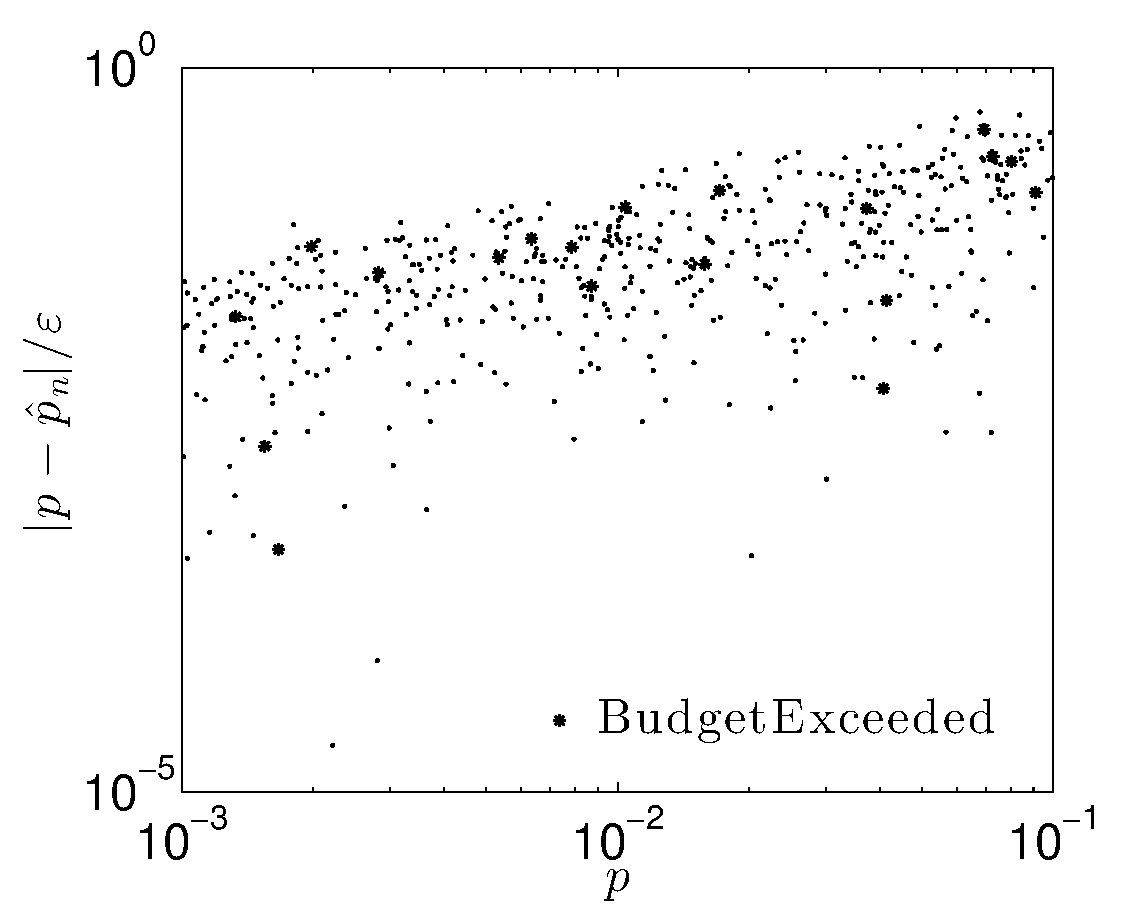
\includegraphics[width=9cm]{abs.eps} % requires the graphicx package
    \caption{Ratio of the actual absolute error to the error tolerance from {\tt meanMCber\_g} versus $p$, for different random samples of $\Ber(p)$ random variables.}
    \label{fig:abserrex}
 \end{figure}

 
While it is encouraging to see that {\tt meanMCber\_g} provides the correct answer in all cases, it is concerning that {\tt meanMCber\_g} is rather conservative for small $p$.  This is due to the fact that the error of $\hp_n$ using $n$ samples is expected to be proportional to $\sqrt{\var(Y)/n}=\sqrt{p(1-p)/n}$.  Even though the error is small for small $p$, our algorithm does not take advantage of that fact.  To do so will require at least a loose lower bound on $p$ at the same time that the algorithm is trying to determine the sample size needed to estimate $p$ carefully.

\Subsection{Test on the relative error criterion}
Another numerical experiment was done with the following parameters:
\begin{itemize}
\item $p$ are given and $\log_{10} p \sim U [-3,-1]$
\item $\varepsilon_r$ are given and random chosen with the distribution $\log_{10} \varepsilon_r \sim U[-2,-1]$
\end{itemize}
  \begin{figure}[htbp]
    \centering
    \includegraphics[width=9cm]{rel.eps} % requires the graphicx package
    \caption{The true relative error/relative error tolerance for different p}
    \label{fig:relerrex}
 \end{figure}
  Similarly, 500 replications were done with random chosen relative error tolerance $\varepsilon_r$ and Bernoulli random variables with random chosen true mean, $p$. In the figure it show that, when $p$ is small, it is more likely to have the sample budget exceeded, as it will be more difficult to estimate the mean with a smaller $p$ than with a larger $p$ with a given relative error tolerance. In more details, we want the condition \eqref{probrel} to be satisfied, there is a denominator which is between $0$ and $1$,  when it gets smaller, we will need a larger sample size to meet this condition.

\Subsection{CLT \& Hoeffding's Inequality Confidence Interval Cost Comparison}
By using Hoeffding's Inequality to construct guaranteed fixed-width confidence interval, we definitely incur additional cost compared to an approximate CLT confidence interval.  The ratio of this cost is 
\begin{equation}
\frac{n_{\Hoeff}}{n_{\CLT}} = \frac{\left \lceil \log(2/\alpha)/{2\varepsilon^2} \right \rceil}{\left \lceil{ \Phi^{-1}(1-\alpha/2)}/{4 \varepsilon^2}\right\rceil} \approx  \frac{2\log(2/\alpha)}{\Phi^{-1}(1-\alpha/2)}.
\end{equation}
This ratio essentially depends on the uncertainty level $\alpha$ and is plotted in Figure \ref{fig:ratiovsalpha}. For $\alpha$ between $0.01\%$ to $10\%$ this ratio is between 3.64 to 5.09, which we believe is a reasonable price to pay for the added certainty of {\tt meanMCber\_g}.

  \begin{figure}[htbp]
    \centering
    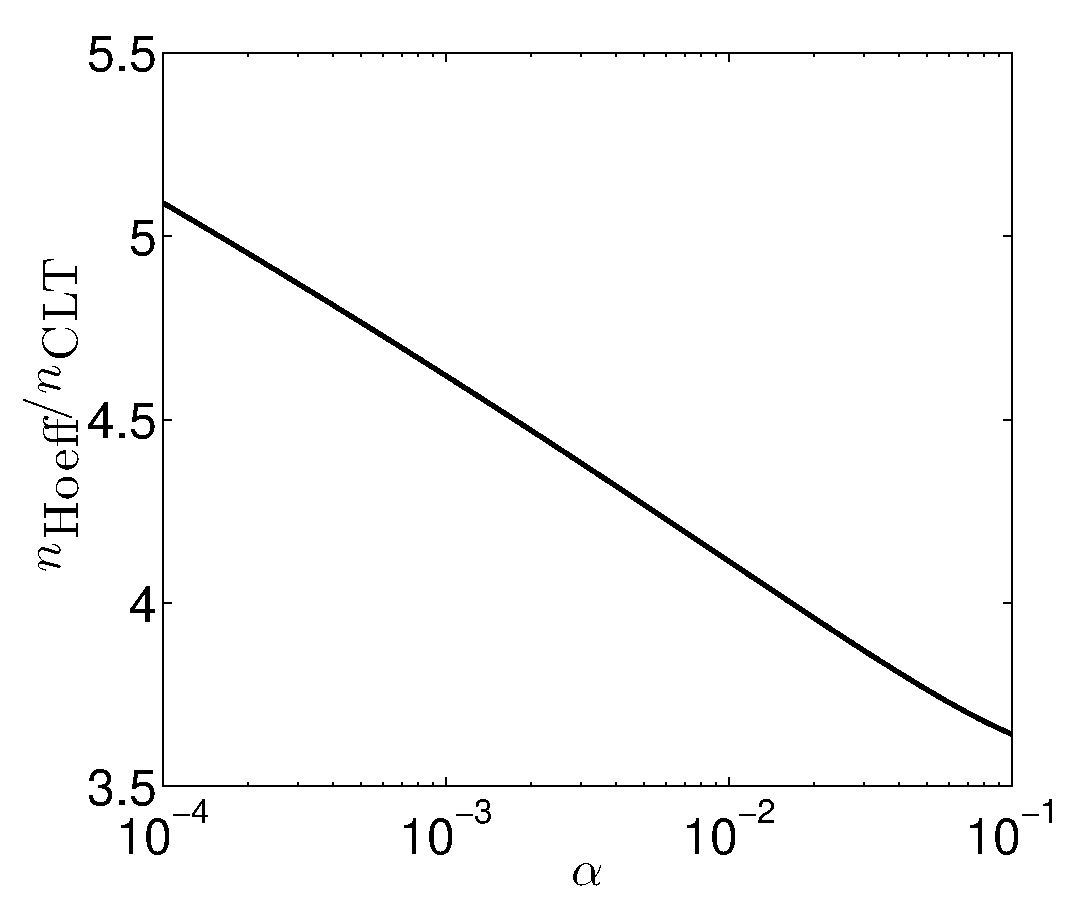
\includegraphics[width=8cm]{plotHoeffCLTr.eps} % requires the graphicx package
    \caption{The computational cost ratio of using Hoeffding's Inequality and the CLT to construct a fixed-width confidence interval.}
    \label{fig:ratiovsalpha}
 \end{figure}
 
 \Chapter{Guaranteed Automatic Integration Library}\label{chapter:gail}
 
Guaranteed Automatic Integration Library (GAIL) \cite{GAIL_2_1} is a MATLAB toolbox created and developed by a group of researchers including Sou-Cheng T. Choi, Yuhan Ding, Fred J. Hickernell, Lan Jiang, Ll\'{u}ıs Antoni Ji\'{m}enez Rugama, Xin Tong, Yizhi Zhang and Xuan Zhou. It is a suite of algorithms including automatic and adaptive univariate function approximation ({\tt funappx\_g}), function minimization using linear splines ({\tt funmin\_g}), one-dimensional numerical integration using trapezoidal rule ({\tt integral\_g}) and mean estimation and numerical integration using Monte Carlo methods ({\tt meanMC\_g},{\tt cubMC\_g} and {\tt meanMCBer\_g}). This purpose is to create a reliable and robust open source MATLAB package, following the philosophy of reproducible research (RR) championed by Claerbout \cite{Claerbout10} and Donoho\cite{BuckheitDonoho95} and developing supportable scientific software (SSS) that promote reliable reproducible research (RRR). In the next section, we will describe the structure of GAIL and the way we develop it.

\begin{sidewaysfigure}[hb]
\centering
\includegraphics[width=8in]
{GAILTree.pdf} 
\caption{GAIL directory hierarchy \label{GAILTree}}
\end{sidewaysfigure}

\Section{Introduction to GAIL}

Figure \ref{GAILTree} shows the structure and hierarchy of the toolbox GAIL. It contains several levels of directories.
\begin{itemize}
\item Documentations: includes the scripts that generate the html supporting and explaining the algorithms.
\item Papers: includes the published papers related to GAIL.
\item Algorithms: the core part of GAIL, which included the ten algorithms shown in Figure \ref{GAILTree}.
\item Tests: includes doctest and unittest for all the algorithms.
\item Workouts: several examples are tested here.
\item Output Files: the output files generated from workouts and papers.
\item Third Party: the useful third party tools are added including doctest package and chebfun package.
\end{itemize}

 \Subsection{Downloads}
GAIL can be downloaded from

\url{http://code.google.com/p/gail/}

Alternatively, you can get a local copy of the GAIL repository with this command:
\begin{lstlisting}
git clone https://github.com/GailGithub/GAIL_Dev.git
\end{lstlisting}

You will need to install MATLAB 7 or a later version.


\Subsection{Documentation}
Detailed documentation is available at GAIL Matlab/Documentation directory.

\Subsection{Algorithms}
GAIL Version 2.1 \cite{GAIL_2_1} includes the following eight algorithms:
\begin{itemize}
\item {\tt funappx\_g}: 1-D function approximation on a bounded interval with local adaption.
\item {\tt funmin\_g}: global univariate function minimization on a bounded interval.
\item {\tt integral\_g}: 1-D numerical integration on a bounded interval based on Trapezoidal rule.
\item {\tt cubLattice\_g}: Numerical integration via Quasi-Monte Carlo method using rank-1 Lattices.
\item {\tt cubSobol\_ g}: Numerical integration via Quasi-Monte Carlo method using Sobol’ points.
\item {\tt meanMCabs\_g}: Monte Carlo method for estimating mean of a random variable with an absolute error tolerance.
\item {\tt meanMC\_g}: Monte Carlo method for estimating mean of a random variable with a generalized error tolerance.
\item {\tt cubMCabs\_g}: Monte Carlo method for numerical integration with an absolute error tolerance.
\item {\tt cubMC\_g}: Monte Carlo method for numerical integration with a generalized error tolerance.
\item  {\tt meanMCBer\_g}: Monte Carlo method to estimate the mean of a Bernoulli random variable.
\end{itemize}

\Subsection{Installation Instruction}
\begin{enumerate}
\item Unzip the contents of the zip file to a directory and maintain the existing directory and subdirectory structure. (Please note: If you install into the toolbox sub-directory of the MATLAB program hierarchy, you will need to click the button "Update toolbox path cache" from the File/Preferences... dialog in MATLAB.)
\item In MATLAB, add the GAIL directory to your path. This can be done by running GAIL Install.m. Alternatively, this can be done by selecting “File/Set Path...” from the main or Command window menus, or with the command pathtool. We recommend that you select the “Save” button on this dialog so that GAIL is on the path automatically in future MATLAB sessions.
\item To check if you have installed GAIL successfully, type {\tt help meanMC\_g} to see if its documentation shows up.
\end{enumerate}

Alternatively, you could do this:
\begin{enumerate}
\item Download {\tt DownloadInstallGail 2\_1.m} and put it where you want GAIL to be installed.
\item Execute it in MATLAB.
\end{enumerate}

To uninstall GAIL, execute {\tt GAIL\_Uninstall}.

\Subsection{Tests}
Two tests are provided here, doctest and unittest, for each of the algorithms.
\begin{itemize}
\item To run doctests, simply call {\tt doctest meanMC\_g}
\item To run unittest, call {\tt run(ut\_meanMC\_g)}. Please note, unittest is only supported for MTALAB version 8 or later.
\end{itemize}


\Chapter{Conclusion}\label{chapter:comclusion}

In this thesis, we studied several algorithms that estimate the mean of a random variable, perform numerical integration via Monte-Carlo sampling and estimate the probability. All these algorithms carry guarantee that the estimators satisfy fixed width confidence interval conditions.

With the given knowledge of bounded kurtosis condition in \eqref{def:boundedkurtosis}, We first introduced two algorithms, {\tt meanMCabs\_g} in Algorithm \ref{alg:meanMCabsg} and {\tt cubMCabs\_g} in Algorithm \ref{alg:cubMCabsg}, which estimate the mean of a random variable and estimate the integral to some prescribed absolute error tolerance $\varepsilon_a$. A probabilistic upper bound on the cost are calculated in Section \ref{sec:meanMCabsgcost}. Several numerical examples are performed including integrating a single hump \eqref{GaussianTestFun} and the Keister test function \eqref{KeisterTestFun}, estimating the Asian geometric mean call option in Subsection \ref{subsec:asiancallopt}. Time and accuracy are recorded and plotted to compare these two algorithms with other algorithms including {\tt integral} in MATLAB, {\tt Chebfun} \cite{Chebfun14}, {\tt cubSobol\_g} and {\tt cubLattice\_g} in GAIL \cite{GAIL_2_1}, which are shown Figure \ref{fig:GaussianTestFun}, \ref{fig:GaussianTestFunHD}, \ref{fig:keistertestfunabstol} and \ref{fig:GeoMeanAsianOptionabstol}.

If one want our answer correct to some specified relative error tolerance $\varepsilon_r$, or some hybrid error criterion defined in Definition \ref{def:tolfun}, another two algorithms are provided. They are iteratively estimating the mean or the integral until a stopping criterion is reached. In details, {\tt meanMC\_g} in Algorithm \ref{alg:meanMCg} is used to estimate the mean of a random variable $Y$ to some generalized error tolerance $\tol(\varepsilon_a, \varepsilon_r)$ with a high confidence level; {\tt cubMC\_g} in Algorithm \ref{alg:cubMCg} uses the same idea to do numerical integration and it carries the guarantee that the estimator $\tilde{I}$ satisfies the fixed width confidence interval condition \eqref{cubMCgCI}. Computational cost upper bound is derived in Section \ref{sec:meanmcgcost}. Several numerical examples are given in Section \ref{sec:cubmcgnumericalexample} with a single hump integrand \eqref{GaussiankerTestFun}, the Keister test function \eqref{KeisterTestFun} and Multivariate Normal Probability function \eqref{MVNP}. Time and accuracy results are recorded and plotted with the comparison with several different algorithms.

Sometime, one may be interested in estimating the probability. Given a Bernoulli random variable, which only have value 1 and 0, with the distribution $\Pr(Y =1) = p$, one may want to estimate this value $p$ to some specified absolute error tolerance $\varepsilon_a$ or relative error tolerance $\varepsilon_r$. In Chapter \ref{chapter:meanMCberg}, we suggest a way to estimate $p$ to a prescribed absolute error tolerance in Algorithm \ref{algabs} and to a relative error tolerance $\varepsilon_r$ in Algorithm \ref{algrel}. Computational cost and numerical examples followed.


\Chapter{Future work}\label{chapter: future work}

We believe that the guaranteed adaptive algorithms are of great interests to the recent practitioners and researchers, as we have suggested a few ways to solve the problems like numerical integration using 1-D trapezoid rule {\tt integral\_g} , unitvariate function approximation {\tt funappx\_g} and {\tt funappxglobal\_g}, Monte Carlo methods for evaluating the mean of a random variable {\tt meanMCabs\_g} and {\tt meanMC\_g}, numerical integration via Monte Carlo {\tt cubMCabs\_g} and {\tt cubMC\_g}, probability estimation using Bernoulli random variables {\tt meanMCber\_g}. These works have been published in \cite{CDHHZ13} and \cite{HJLO12}. Also, we believe these the algorithms followed by theoretical research should be carefully implemented, documented and published. Thus, we have developed our MATLAB toolbox: Guaranteed Automatic Integration Library (GAIL) \cite{GAIL_2_1}. The work in this article has became part of this toolbox. Some possible future work that could be done will be explained in the following paragraphs.

As {\tt cubMC\_g} does Monte Carlo method for numerical integration, some variance reduction techniques could be applied to make the simulation more efficient. Such techniques includes control variate, importance sampling and Quasi Monte Carlo(QMC) methods. As one of our colleagues has been working on guaranteed adaptive quasi Monte Carlo method using Sobol' points \cite{Sobol67} and Lattice points, two algorithms {\tt cubSobol\_g} and {\tt cubLattice\_g} are the ones in GAIL. The other two variance reduction techniques may be the possible future work.

For the algorithms {\tt meanMCabs\_g} and {\tt meanMC\_g}, the cost upper bound has been derived, the lower bound derivation is another possible research area. More practical real work examples could be implemented to test our guaranteed Monte Carlo methods in GAIL.

The Algorithm \ref{algabs} and \ref{algrel} will do the calculation in order to meet either absolute error tolerance or relative error tolerance, another area for further research is to set the tolerance as: $\text{tol} = \max(\varepsilon_a, \varepsilon_r p)$, which may be called as a generalized error tolerance or a hybrid error tolerance. In this way, user will provide both of the tolerance and the algorithm will determine which one will be met first. As the upper bound of the algorithm \ref{algrel} is given in theorem \ref{costupperboundrel}, the lower bound of the cost is also an area for further research. 

%\appendix
%
%\Appendix{MATLAB Code of meanMCabs\_g}
%\lstinputlisting{meanMCabs_g.m}
%\Appendix{MATLAB Code of cubMCabs\_g}
%\lstinputlisting{cubMCabs_g.m}
%\Appendix{MATLAB Code of meanMC\_g}
%\lstinputlisting{meanMC_g.m}
%%\input{meanMC_g.m}
%\Appendix{MATLAB Code of cubMC\_g}
%\lstinputlisting{cubMC_g.m}
%\Appendix{MATLAB Code of meanMCber\_g}
%\lstinputlisting{meanMCber_g.m}

\bibliographystyle{alpha}
\bibliography{Ljiang}

%\input{meanMCgCode}
%\input{cubMCgCode}
%\input{meanMCBergCode}
\end{document}  % end of document
